% Options for packages loaded elsewhere
\PassOptionsToPackage{unicode}{hyperref}
\PassOptionsToPackage{hyphens}{url}
%
\documentclass[
]{article}
\usepackage{amsmath,amssymb}
\usepackage{lmodern}
\usepackage{iftex}
\ifPDFTeX
  \usepackage[T1]{fontenc}
  \usepackage[utf8]{inputenc}
  \usepackage{textcomp} % provide euro and other symbols
\else % if luatex or xetex
  \usepackage{unicode-math}
  \defaultfontfeatures{Scale=MatchLowercase}
  \defaultfontfeatures[\rmfamily]{Ligatures=TeX,Scale=1}
\fi
% Use upquote if available, for straight quotes in verbatim environments
\IfFileExists{upquote.sty}{\usepackage{upquote}}{}
\IfFileExists{microtype.sty}{% use microtype if available
  \usepackage[]{microtype}
  \UseMicrotypeSet[protrusion]{basicmath} % disable protrusion for tt fonts
}{}
\makeatletter
\@ifundefined{KOMAClassName}{% if non-KOMA class
  \IfFileExists{parskip.sty}{%
    \usepackage{parskip}
  }{% else
    \setlength{\parindent}{0pt}
    \setlength{\parskip}{6pt plus 2pt minus 1pt}}
}{% if KOMA class
  \KOMAoptions{parskip=half}}
\makeatother
\usepackage{xcolor}
\usepackage[margin=1in]{geometry}
\usepackage{color}
\usepackage{fancyvrb}
\newcommand{\VerbBar}{|}
\newcommand{\VERB}{\Verb[commandchars=\\\{\}]}
\DefineVerbatimEnvironment{Highlighting}{Verbatim}{commandchars=\\\{\}}
% Add ',fontsize=\small' for more characters per line
\usepackage{framed}
\definecolor{shadecolor}{RGB}{248,248,248}
\newenvironment{Shaded}{\begin{snugshade}}{\end{snugshade}}
\newcommand{\AlertTok}[1]{\textcolor[rgb]{0.94,0.16,0.16}{#1}}
\newcommand{\AnnotationTok}[1]{\textcolor[rgb]{0.56,0.35,0.01}{\textbf{\textit{#1}}}}
\newcommand{\AttributeTok}[1]{\textcolor[rgb]{0.77,0.63,0.00}{#1}}
\newcommand{\BaseNTok}[1]{\textcolor[rgb]{0.00,0.00,0.81}{#1}}
\newcommand{\BuiltInTok}[1]{#1}
\newcommand{\CharTok}[1]{\textcolor[rgb]{0.31,0.60,0.02}{#1}}
\newcommand{\CommentTok}[1]{\textcolor[rgb]{0.56,0.35,0.01}{\textit{#1}}}
\newcommand{\CommentVarTok}[1]{\textcolor[rgb]{0.56,0.35,0.01}{\textbf{\textit{#1}}}}
\newcommand{\ConstantTok}[1]{\textcolor[rgb]{0.00,0.00,0.00}{#1}}
\newcommand{\ControlFlowTok}[1]{\textcolor[rgb]{0.13,0.29,0.53}{\textbf{#1}}}
\newcommand{\DataTypeTok}[1]{\textcolor[rgb]{0.13,0.29,0.53}{#1}}
\newcommand{\DecValTok}[1]{\textcolor[rgb]{0.00,0.00,0.81}{#1}}
\newcommand{\DocumentationTok}[1]{\textcolor[rgb]{0.56,0.35,0.01}{\textbf{\textit{#1}}}}
\newcommand{\ErrorTok}[1]{\textcolor[rgb]{0.64,0.00,0.00}{\textbf{#1}}}
\newcommand{\ExtensionTok}[1]{#1}
\newcommand{\FloatTok}[1]{\textcolor[rgb]{0.00,0.00,0.81}{#1}}
\newcommand{\FunctionTok}[1]{\textcolor[rgb]{0.00,0.00,0.00}{#1}}
\newcommand{\ImportTok}[1]{#1}
\newcommand{\InformationTok}[1]{\textcolor[rgb]{0.56,0.35,0.01}{\textbf{\textit{#1}}}}
\newcommand{\KeywordTok}[1]{\textcolor[rgb]{0.13,0.29,0.53}{\textbf{#1}}}
\newcommand{\NormalTok}[1]{#1}
\newcommand{\OperatorTok}[1]{\textcolor[rgb]{0.81,0.36,0.00}{\textbf{#1}}}
\newcommand{\OtherTok}[1]{\textcolor[rgb]{0.56,0.35,0.01}{#1}}
\newcommand{\PreprocessorTok}[1]{\textcolor[rgb]{0.56,0.35,0.01}{\textit{#1}}}
\newcommand{\RegionMarkerTok}[1]{#1}
\newcommand{\SpecialCharTok}[1]{\textcolor[rgb]{0.00,0.00,0.00}{#1}}
\newcommand{\SpecialStringTok}[1]{\textcolor[rgb]{0.31,0.60,0.02}{#1}}
\newcommand{\StringTok}[1]{\textcolor[rgb]{0.31,0.60,0.02}{#1}}
\newcommand{\VariableTok}[1]{\textcolor[rgb]{0.00,0.00,0.00}{#1}}
\newcommand{\VerbatimStringTok}[1]{\textcolor[rgb]{0.31,0.60,0.02}{#1}}
\newcommand{\WarningTok}[1]{\textcolor[rgb]{0.56,0.35,0.01}{\textbf{\textit{#1}}}}
\usepackage{graphicx}
\makeatletter
\def\maxwidth{\ifdim\Gin@nat@width>\linewidth\linewidth\else\Gin@nat@width\fi}
\def\maxheight{\ifdim\Gin@nat@height>\textheight\textheight\else\Gin@nat@height\fi}
\makeatother
% Scale images if necessary, so that they will not overflow the page
% margins by default, and it is still possible to overwrite the defaults
% using explicit options in \includegraphics[width, height, ...]{}
\setkeys{Gin}{width=\maxwidth,height=\maxheight,keepaspectratio}
% Set default figure placement to htbp
\makeatletter
\def\fps@figure{htbp}
\makeatother
\setlength{\emergencystretch}{3em} % prevent overfull lines
\providecommand{\tightlist}{%
  \setlength{\itemsep}{0pt}\setlength{\parskip}{0pt}}
\setcounter{secnumdepth}{-\maxdimen} % remove section numbering
\ifLuaTeX
  \usepackage{selnolig}  % disable illegal ligatures
\fi
\IfFileExists{bookmark.sty}{\usepackage{bookmark}}{\usepackage{hyperref}}
\IfFileExists{xurl.sty}{\usepackage{xurl}}{} % add URL line breaks if available
\urlstyle{same} % disable monospaced font for URLs
\hypersetup{
  pdftitle={FM project},
  hidelinks,
  pdfcreator={LaTeX via pandoc}}

\title{FM project}
\author{}
\date{\vspace{-2.5em}2023-04-25}

\begin{document}
\maketitle

Reads

\url{https://www.eia.gov/todayinenergy/detail.php?id=55920\#}:\textasciitilde:text=Europe\%20became\%20the\%20primary\%20destination,U.S.\%20LNG\%20exports\%20to\%20Europe.

\hypertarget{analysing-u.s.-energy-exports}{%
\subsection{Analysing U.S. energy
exports}\label{analysing-u.s.-energy-exports}}

\hypertarget{introduction}{%
\subsubsection{1.Introduction}\label{introduction}}

Energy commodities play a pivotal role in the global economy, as they
are essential for economic growth and development. They are required for
transportation, manufacturing, heating, cooling, and many other critical
activities that drive economic activity.

The production, consumption, and trade of energy commodities have
significant impacts on the global economy. The prices of energy
commodities are influenced by supply and demand factors, geopolitical
tensions, weather events, and technological advances.

The recent COVID-19 pandemic and the war in Ukraine have created
unprecedented changes in the energy market, and understanding the impact
of these events is crucial for policymakers, analysts, and investors.
This study aims to examine how the Russian war on Ukraine affected
energy exports of the United States to the OECD Europe countries.

OECD Europe was selected as the region, as because of geographical and
historical relations it was most influenced region by the Russian war on
Ukraine. The United States has been chosen as the focus because it is
one of the leading producers and exporters of energy commodities, and
its export trends have significant implications for the global energy
market. Moreover, the United States serves as a significant alternative
for OECD Europe countries to turn to after the imposition of sanctions
on Russia.

In this study, we will analyze the impact of the war in Ukraine on US
energy exports to OECD Europe. Specifically, we will focus on three main
energy products: crude oil, petroleum products, and natural gas. By
examining trends in these exports, we can better understand how the
geopolitical events in Ukraine have affected the energy market in
Europe. Additionally, we will investigate changes in OECD Europe's
dependence on Russian gas to see how energy dynamics in the region have
shifted.

\hypertarget{time-series-graphics}{%
\subsubsection{2. Time Series Graphics}\label{time-series-graphics}}

In this section of the report, we will be creating time series graphics
using various techniques such as time plots, seasonal plots, seasonal
subseries plots, and ACF(). These plots will provide insights into the
different time series in the dataset and help us understand their
characteristics, such as seasonality, trend, and cyclicity. We will also
look for unusual observations and changing patterns over time and
explore the differences between the series in terms of these features.
Additionally, for this analysis, we have decided to focus on three
specific time series: US exports of Natural Gas to OECD, US Exports of
Crude Oil to OECD, and US exports of Petroleum products to OECD. We will
create the same types of graphs for all of these time series, including
time plots, seasonal plots, seasonal subseries plots, and ACF plots.
These time series span the last ten years from 2013 to 2023. Through
these analyses, we aim to gain insights into the seasonality, cyclicity,
trend, unusual observations, changing patterns, and differences between
these time series, and determine if any of the series resemble a white
noise process. By analyzing these time series graphics, we can gain a
better understanding of the data and identify any potential patterns or
anomalies that may exist within it.

\hypertarget{dataset}{%
\paragraph{2.1 Dataset}\label{dataset}}

The data sets utilized in this study consist of monthly observations of
Country's reliance on Russian oil products, USA's natural gas exports by
country, USA's total crude oil exports by destination, and USA's
petroleum products exports by destination.

Our primary source of data is the U.S. Energy Information Administration
(EIA), an independent organization that collects, analyzes, and
disseminates data and information related to energy production,
consumption, and distribution in the United States. Also, for the
purpose of this study we are using data from the International Energy
Agency (IEA), which is an intergovernmental organization that was
established in 1974 to promote global cooperation on energy issues.

In case of data on reliance on Russian Oil the dataset contains monthly
total oil imports from Russia as a percentage of total oil imports for a
selected group of European countries belonging to the Organization for
Economic Co-operation and Development (OECD) from January 1990 to
October 2022. The dataset includes the date, country name, and the
percentage of total oil imports that came from Russia for each
observation.

In this section, we will analyze three datasets that pertain to US
exports of Crude oil, Petroleum Products, and Natural Gas, all measured
in barrels. Prior to converting the data to tsibble format, we performed
data cleaning and formatting. To simplify the data, we converted each
dataset to have the same structure, with three columns: date,
destination country, and the amount exported. After standardizing the
format, we converted each dataset to tsibble format. We then filtered
the data to only include countries that are part of the OECD and
summarized the results based on the amount exported on each date,
removing country names and leaving only the date and amount exported.
Finally, we merged all three tsibble tables into one by using the left
join function and pivoting the data, resulting in a final time series
that represents US exports of the three different products in barrels to
OECD countries. The tsibble contains three columns: Date, Export Type,
and Amount.

\begin{Shaded}
\begin{Highlighting}[]
\FunctionTok{library}\NormalTok{(fpp3)}
\FunctionTok{library}\NormalTok{(tidyverse)}
\FunctionTok{library}\NormalTok{(ggplot2)}
\FunctionTok{library}\NormalTok{(dplyr)}
\FunctionTok{library}\NormalTok{(tidyr)}
\FunctionTok{library}\NormalTok{(lubridate)}
\FunctionTok{library}\NormalTok{(scales)}

\CommentTok{\#Total Crude Oil Exports by Destination}


\NormalTok{raw\_crude\_oil }\OtherTok{\textless{}{-}} \FunctionTok{read\_csv}\NormalTok{(}\StringTok{"https://raw.githubusercontent.com/edb{-}313/Energy{-}trade{-}forecasting/main/Data/csv/Total\%20Crude\%20Oil\%20Exports\%20by\%20Destination\_EIA.csv"}\NormalTok{, }\AttributeTok{skip =} \DecValTok{2}\NormalTok{,)}


\CommentTok{\#Leaving only country names in column names}

\FunctionTok{names}\NormalTok{(raw\_crude\_oil)[}\SpecialCharTok{{-}}\DecValTok{2}\NormalTok{] }\OtherTok{\textless{}{-}} \FunctionTok{str\_replace\_all}\NormalTok{(}\FunctionTok{names}\NormalTok{(raw\_crude\_oil)[}\SpecialCharTok{{-}}\DecValTok{2}\NormalTok{],}
                                            \FunctionTok{c}\NormalTok{(}\StringTok{"U.S. Exports to "} \OtherTok{=} \StringTok{""}\NormalTok{,}
                                              \StringTok{" of Crude Oil }\SpecialCharTok{\textbackslash{}\textbackslash{}}\StringTok{(Thousand Barrels}\SpecialCharTok{\textbackslash{}\textbackslash{}}\StringTok{)"} \OtherTok{=} \StringTok{""}\NormalTok{))}

\CommentTok{\#Pivoting (switching) columns starting from 2 column to rows}

\NormalTok{crude\_oil }\OtherTok{\textless{}{-}}\NormalTok{ raw\_crude\_oil }\SpecialCharTok{\%\textgreater{}\%} 
  \FunctionTok{pivot\_longer}\NormalTok{(}\AttributeTok{cols =} \SpecialCharTok{{-}}\NormalTok{Date,}
               \AttributeTok{names\_to =} \StringTok{\textquotesingle{}Destination country\textquotesingle{}}\NormalTok{,}
               \AttributeTok{values\_to =} \StringTok{\textquotesingle{}Amount of Crude Oil (Thousand Barrels)\textquotesingle{}}\NormalTok{)}



\CommentTok{\#Filtering out values where Date is \textquotesingle{}NA\textquotesingle{}}

\NormalTok{crude\_oil }\OtherTok{\textless{}{-}}\NormalTok{ crude\_oil }\SpecialCharTok{\%\textgreater{}\%}
  \FunctionTok{drop\_na}\NormalTok{(Date) }\SpecialCharTok{\%\textgreater{}\%}
  \FunctionTok{mutate}\NormalTok{(}\AttributeTok{Date =} \FunctionTok{as.Date}\NormalTok{(Date))}

\CommentTok{\#Fixing date format, replacing \textquotesingle{}na\textquotesingle{} values with 0}

\NormalTok{crude\_oil}\SpecialCharTok{$}\NormalTok{Date }\OtherTok{\textless{}{-}} \FunctionTok{as.Date}\NormalTok{(crude\_oil}\SpecialCharTok{$}\NormalTok{Date)}
\NormalTok{crude\_oil}\SpecialCharTok{$}\StringTok{\textasciigrave{}}\AttributeTok{Amount of Crude Oil (Thousand Barrels)}\StringTok{\textasciigrave{}} \OtherTok{\textless{}{-}} \FunctionTok{replace\_na}\NormalTok{(crude\_oil}\SpecialCharTok{$}\StringTok{\textasciigrave{}}\AttributeTok{Amount of Crude Oil (Thousand Barrels)}\StringTok{\textasciigrave{}}\NormalTok{, }\DecValTok{0}\NormalTok{)}

\CommentTok{\#Setting up the tsibble}

\NormalTok{ts\_crude\_oil }\OtherTok{\textless{}{-}}\NormalTok{ crude\_oil }\SpecialCharTok{\%\textgreater{}\%}
  \FunctionTok{mutate}\NormalTok{(}\AttributeTok{Date =} \FunctionTok{yearmonth}\NormalTok{(Date)) }\SpecialCharTok{\%\textgreater{}\%} 
  \FunctionTok{as\_tsibble}\NormalTok{(}
    \AttributeTok{index =}\NormalTok{ Date, }
    \AttributeTok{key =} \StringTok{\textasciigrave{}}\AttributeTok{Destination country}\StringTok{\textasciigrave{}}
\NormalTok{  )}



\CommentTok{\#OECD Europe Countries vector}

\NormalTok{oecd\_europe }\OtherTok{\textless{}{-}} \FunctionTok{c}\NormalTok{(}\StringTok{"Austria"}\NormalTok{, }\StringTok{"Belgium"}\NormalTok{, }\StringTok{"Czech Republic"}\NormalTok{, }\StringTok{"Denmark"}\NormalTok{, }\StringTok{"Estonia"}\NormalTok{,}
                 \StringTok{"Finland"}\NormalTok{, }\StringTok{"France"}\NormalTok{, }\StringTok{"Germany"}\NormalTok{, }\StringTok{"Greece"}\NormalTok{, }\StringTok{"Hungary"}\NormalTok{, }\StringTok{"Iceland"}\NormalTok{,}
                 \StringTok{"Ireland"}\NormalTok{, }\StringTok{"Italy"}\NormalTok{, }\StringTok{"Latvia"}\NormalTok{, }\StringTok{"Lithuania"}\NormalTok{, }\StringTok{"Luxembourg"}\NormalTok{,}
                 \StringTok{"Netherlands"}\NormalTok{, }\StringTok{"Norway"}\NormalTok{, }\StringTok{"Poland"}\NormalTok{, }\StringTok{"Portugal"}\NormalTok{, }\StringTok{"Slovak Republic"}\NormalTok{,}
                 \StringTok{"Slovenia"}\NormalTok{, }\StringTok{"Spain"}\NormalTok{, }\StringTok{"Sweden"}\NormalTok{, }\StringTok{"Switzerland"}\NormalTok{, }\StringTok{"Turkey"}\NormalTok{,}
                 \StringTok{"United Kingdom"}\NormalTok{)}

\CommentTok{\#filtering out only relevant values}

\NormalTok{oecd\_crude\_oil }\OtherTok{\textless{}{-}}\NormalTok{ ts\_crude\_oil }\SpecialCharTok{\%\textgreater{}\%}
  \FunctionTok{filter}\NormalTok{(}\StringTok{\textasciigrave{}}\AttributeTok{Destination country}\StringTok{\textasciigrave{}} \SpecialCharTok{\%in\%}\NormalTok{ oecd\_europe) }\SpecialCharTok{\%\textgreater{}\%} 
  \FunctionTok{filter}\NormalTok{(Date }\SpecialCharTok{\textgreater{}=} \FunctionTok{as.Date}\NormalTok{(}\StringTok{"2014{-}04{-}15"}\NormalTok{), Date }\SpecialCharTok{\textless{}=} \FunctionTok{as.Date}\NormalTok{(}\StringTok{"2023{-}01{-}15"}\NormalTok{)) }

\NormalTok{oecd\_crude\_oil\_agg }\OtherTok{\textless{}{-}}\NormalTok{ oecd\_crude\_oil }\SpecialCharTok{\%\textgreater{}\%}
  \FunctionTok{index\_by}\NormalTok{(Date) }\SpecialCharTok{\%\textgreater{}\%}
  \FunctionTok{summarize\_at}\NormalTok{(}\FunctionTok{vars}\NormalTok{(}\StringTok{\textasciigrave{}}\AttributeTok{Amount of Crude Oil (Thousand Barrels)}\StringTok{\textasciigrave{}}\NormalTok{), sum) }\SpecialCharTok{\%\textgreater{}\%}
  \FunctionTok{ungroup}\NormalTok{()}


\DocumentationTok{\#\#\#\#\#\#\#\#\#\#\#\#\#\#\#\#\#\#\#\#\#\#\#\#\#\#\#\#\#\#\#\#\#\#\#\#\#\#\#\#\#\#\#\#\#\#\#\#\#\#\#\#\#\#\#\#\#\#\#\#\#\#\#\#\#\#\#\#\#\#\#\#\#\#\#\#\#\#\#\#}

\CommentTok{\#Total Oil Products Exports by Destination}

\NormalTok{raw\_oil\_prod }\OtherTok{\textless{}{-}} \FunctionTok{read\_csv}\NormalTok{(}\StringTok{"https://raw.githubusercontent.com/edb{-}313/Energy{-}trade{-}forecasting/main/Data/csv/Total\%20Oil\%20Products\%20Exports\%20by\%20Destination\_EIA.csv"}\NormalTok{,  }\AttributeTok{skip =} \DecValTok{2}\NormalTok{,)}

\FunctionTok{names}\NormalTok{(raw\_oil\_prod)[}\SpecialCharTok{{-}}\DecValTok{2}\NormalTok{] }\OtherTok{\textless{}{-}} \FunctionTok{str\_replace\_all}\NormalTok{(}\FunctionTok{names}\NormalTok{(raw\_oil\_prod)[}\SpecialCharTok{{-}}\DecValTok{2}\NormalTok{],}
                                           \FunctionTok{c}\NormalTok{(}\StringTok{"U.S. Exports to "} \OtherTok{=} \StringTok{""}\NormalTok{,}
                                             \StringTok{" of Total Petroleum Products }\SpecialCharTok{\textbackslash{}\textbackslash{}}\StringTok{(Thousand Barrels}\SpecialCharTok{\textbackslash{}\textbackslash{}}\StringTok{)"} \OtherTok{=} \StringTok{""}\NormalTok{))}
\NormalTok{oil\_prod }\OtherTok{\textless{}{-}}\NormalTok{ raw\_oil\_prod }\SpecialCharTok{\%\textgreater{}\%} 
  \FunctionTok{pivot\_longer}\NormalTok{(}\AttributeTok{cols =} \SpecialCharTok{{-}}\NormalTok{Date,}
               \AttributeTok{names\_to =} \StringTok{\textquotesingle{}Destination country\textquotesingle{}}\NormalTok{,}
               \AttributeTok{values\_to =} \StringTok{\textquotesingle{}Amount of total Petroleum Porducts (Thousand Barrels)\textquotesingle{}}\NormalTok{)}


\NormalTok{oil\_prod}\SpecialCharTok{$}\StringTok{\textasciigrave{}}\AttributeTok{Amount of total Petroleum Porducts (Thousand Barrels)}\StringTok{\textasciigrave{}} \OtherTok{\textless{}{-}} \FunctionTok{replace\_na}\NormalTok{(oil\_prod}\SpecialCharTok{$}\StringTok{\textasciigrave{}}\AttributeTok{Amount of total Petroleum Porducts (Thousand Barrels)}\StringTok{\textasciigrave{}}\NormalTok{, }\DecValTok{0}\NormalTok{)}

\NormalTok{oil\_prod }\OtherTok{\textless{}{-}}\NormalTok{ oil\_prod }\SpecialCharTok{\%\textgreater{}\%} 
  \FunctionTok{drop\_na}\NormalTok{(Date) }\SpecialCharTok{\%\textgreater{}\%} 
  \FunctionTok{mutate}\NormalTok{(}\AttributeTok{Date =} \FunctionTok{as.Date}\NormalTok{(Date))}

\NormalTok{ts\_oil\_prod }\OtherTok{\textless{}{-}}\NormalTok{ oil\_prod }\SpecialCharTok{\%\textgreater{}\%}
  \FunctionTok{mutate}\NormalTok{(}\AttributeTok{Date =} \FunctionTok{yearmonth}\NormalTok{(Date)) }\SpecialCharTok{\%\textgreater{}\%} 
  \FunctionTok{as\_tsibble}\NormalTok{(}
    \AttributeTok{index =}\NormalTok{ Date, }
    \AttributeTok{key =} \StringTok{\textasciigrave{}}\AttributeTok{Destination country}\StringTok{\textasciigrave{}}
\NormalTok{  )}

\NormalTok{oecd\_oil\_prod }\OtherTok{\textless{}{-}}\NormalTok{ ts\_oil\_prod }\SpecialCharTok{\%\textgreater{}\%} 
  \FunctionTok{filter}\NormalTok{(}\StringTok{\textasciigrave{}}\AttributeTok{Destination country}\StringTok{\textasciigrave{}} \SpecialCharTok{\%in\%}\NormalTok{ oecd\_europe) }\SpecialCharTok{\%\textgreater{}\%} 
  \FunctionTok{filter}\NormalTok{(Date }\SpecialCharTok{\textgreater{}=} \FunctionTok{as.Date}\NormalTok{(}\StringTok{"2014{-}05{-}15"}\NormalTok{), Date }\SpecialCharTok{\textless{}=} \FunctionTok{as.Date}\NormalTok{(}\StringTok{"2023{-}01{-}15"}\NormalTok{))}


\NormalTok{oecd\_oil\_prod\_agg }\OtherTok{\textless{}{-}}\NormalTok{ oecd\_oil\_prod }\SpecialCharTok{\%\textgreater{}\%}
  \FunctionTok{index\_by}\NormalTok{(Date) }\SpecialCharTok{\%\textgreater{}\%}
  \FunctionTok{summarize\_at}\NormalTok{(}\FunctionTok{vars}\NormalTok{(}\StringTok{\textasciigrave{}}\AttributeTok{Amount of total Petroleum Porducts (Thousand Barrels)}\StringTok{\textasciigrave{}}\NormalTok{), sum) }\SpecialCharTok{\%\textgreater{}\%}
  \FunctionTok{ungroup}\NormalTok{()}

\DocumentationTok{\#\#\#\#\#\#\#\#\#\#\#\#\#\#\#\#\#\#\#\#\#\#\#\#\#\#\#\#\#\#\#\#\#\#\#\#\#\#\#\#\#\#\#\#\#\#\#\#\#\#\#\#\#\#\#\#\#\#\#\#\#\#\#\#\#\#\#\#\#\#\#\#\#\#\#\#\#\#\#\#}
\CommentTok{\#Reliance on Russian gas}

\NormalTok{raw\_rel\_rusoil }\OtherTok{\textless{}{-}} \FunctionTok{read\_csv}\NormalTok{(}\StringTok{"https://raw.githubusercontent.com/edb{-}313/Energy{-}trade{-}forecasting/main/Data/csv/Monthly\_Reliance\_on\_Russian\_Oil.csv"}\NormalTok{, }\AttributeTok{skip =} \DecValTok{1}\NormalTok{)}

\NormalTok{rel\_rusoil }\OtherTok{\textless{}{-}}\NormalTok{ raw\_rel\_rusoil }\SpecialCharTok{\%\textgreater{}\%} 
  \FunctionTok{pivot\_longer}\NormalTok{(}\AttributeTok{cols =} \SpecialCharTok{{-}}\NormalTok{...}\DecValTok{1}\NormalTok{,}
               \AttributeTok{names\_to =} \StringTok{\textquotesingle{}Date\textquotesingle{}}\NormalTok{,}
               \AttributeTok{values\_to =} \StringTok{\textquotesingle{}Total Oil Imports from Russia / Total Oil Imports (\%)\textquotesingle{}}\NormalTok{)}

\NormalTok{rel\_rusoil }\OtherTok{\textless{}{-}}\NormalTok{ rel\_rusoil }\SpecialCharTok{\%\textgreater{}\%} 
  \FunctionTok{rename}\NormalTok{(}\AttributeTok{Country =}\NormalTok{ ...}\DecValTok{1}\NormalTok{) }\SpecialCharTok{\%\textgreater{}\%} 
  \FunctionTok{mutate}\NormalTok{(}\AttributeTok{Date =}\NormalTok{ lubridate}\SpecialCharTok{::}\FunctionTok{dmy}\NormalTok{(Date)) }\SpecialCharTok{\%\textgreater{}\%} 
  \FunctionTok{select}\NormalTok{(}\StringTok{"Date"}\NormalTok{,}\StringTok{"Country"}\NormalTok{,}\StringTok{"Total Oil Imports from Russia / Total Oil Imports (\%)"}\NormalTok{)}


\NormalTok{ts\_rel\_rusoil }\OtherTok{\textless{}{-}}\NormalTok{ rel\_rusoil }\SpecialCharTok{\%\textgreater{}\%} 
  \FunctionTok{as\_tsibble}\NormalTok{(}
    \AttributeTok{index =}\NormalTok{ Date,}
    \AttributeTok{key =}\NormalTok{ Country)}

\NormalTok{oecd\_relrus }\OtherTok{\textless{}{-}}\NormalTok{ ts\_rel\_rusoil }\SpecialCharTok{\%\textgreater{}\%}
  \FunctionTok{filter}\NormalTok{(Country }\SpecialCharTok{\%in\%}\NormalTok{ oecd\_europe)}

\DocumentationTok{\#\#\#\#\#\#\#\#\#\#\#\#\#\#\#\#\#\#\#\#\#\#\#\#\#\#\#\#\#\#\#\#\#\#\#\#\#\#\#\#\#\#\#\#\#\#\#\#\#\#\#\#\#\#\#\#\#\#\#\#\#\#\#\#\#\#\#\#\#\#\#\#\#\#\#\#\#\#\#\#}
\CommentTok{\#Total Natural Gas Exports by Destination}

\NormalTok{raw\_nat\_gas }\OtherTok{\textless{}{-}} \FunctionTok{read.csv}\NormalTok{(}\StringTok{\textquotesingle{}https://raw.githubusercontent.com/edb{-}313/Energy{-}trade{-}forecasting/main/Data/csv/Natural\%20Gas\%20Exports\%20by\%20Country\_EIA.csv\textquotesingle{}}\NormalTok{,}\AttributeTok{header=}\ConstantTok{TRUE}\NormalTok{ , }\AttributeTok{check.names=}\ConstantTok{FALSE}\NormalTok{, }\AttributeTok{skip =} \DecValTok{2}\NormalTok{)}

\CommentTok{\# drop columns 2{-}3, 6{-}8, 54 and 57{-}72}
\NormalTok{raw\_nat\_gas }\OtherTok{\textless{}{-}} \FunctionTok{subset}\NormalTok{(raw\_nat\_gas, }\AttributeTok{select =} \SpecialCharTok{{-}}\FunctionTok{c}\NormalTok{(}\DecValTok{2}\SpecialCharTok{:}\DecValTok{3}\NormalTok{, }\DecValTok{6}\SpecialCharTok{:}\DecValTok{8}\NormalTok{,}\DecValTok{54}\NormalTok{, }\DecValTok{57}\SpecialCharTok{:}\DecValTok{72}\NormalTok{))}
\NormalTok{raw\_nat\_gas[}\FunctionTok{is.na}\NormalTok{(raw\_nat\_gas)] }\OtherTok{\textless{}{-}} \DecValTok{0}

\CommentTok{\#cimbining exports to the same countries}

\NormalTok{nat\_gas }\OtherTok{\textless{}{-}}\NormalTok{ raw\_nat\_gas }\SpecialCharTok{\%\textgreater{}\%}
  \FunctionTok{mutate}\NormalTok{(}\AttributeTok{Mexico =} \StringTok{\textasciigrave{}}\AttributeTok{U.S. Natural Gas Pipeline Exports to Mexico (MMcf)}\StringTok{\textasciigrave{}} \SpecialCharTok{+} \StringTok{\textasciigrave{}}\AttributeTok{Liquefied U.S. Natural Gas Exports by Truck to Mexico (Million Cubic Feet)}\StringTok{\textasciigrave{}}\NormalTok{,}
         \AttributeTok{Canada =} \StringTok{\textasciigrave{}}\AttributeTok{U.S. Natural Gas Pipeline Exports to Canada (MMcf)}\StringTok{\textasciigrave{}} \SpecialCharTok{+} \StringTok{\textasciigrave{}}\AttributeTok{Liquefied U.S. Natural Gas Exports by Truck to Canada (Million Cubic Feet)}\StringTok{\textasciigrave{}}\NormalTok{)}

\CommentTok{\#removing duplicate columns}

\NormalTok{nat\_gas }\OtherTok{\textless{}{-}}\NormalTok{ nat\_gas[, }\SpecialCharTok{!}\NormalTok{(}\FunctionTok{names}\NormalTok{(nat\_gas) }\SpecialCharTok{\%in\%} \FunctionTok{c}\NormalTok{(}\StringTok{\textquotesingle{}U.S. Natural Gas Pipeline Exports to Mexico (MMcf)\textquotesingle{}}\NormalTok{,}
                                             \StringTok{\textquotesingle{}Liquefied U.S. Natural Gas Exports by Truck to Mexico (Million Cubic Feet)\textquotesingle{}}\NormalTok{,}
                                             \StringTok{\textquotesingle{}U.S. Natural Gas Pipeline Exports to Canada (MMcf)\textquotesingle{}}\NormalTok{,}
                                             \StringTok{\textquotesingle{}Liquefied U.S. Natural Gas Exports by Truck to Canada (Million Cubic Feet)\textquotesingle{}}\NormalTok{))]}

\CommentTok{\#cleaning column names}

\FunctionTok{colnames}\NormalTok{(nat\_gas) }\OtherTok{\textless{}{-}} \FunctionTok{gsub}\NormalTok{(}\AttributeTok{pattern =} \StringTok{".*(to}\SpecialCharTok{\textbackslash{}\textbackslash{}}\StringTok{s)"}\NormalTok{, }\StringTok{""}\NormalTok{, }\FunctionTok{colnames}\NormalTok{(nat\_gas))}
\FunctionTok{colnames}\NormalTok{(nat\_gas) }\OtherTok{\textless{}{-}} \FunctionTok{gsub}\NormalTok{(}\StringTok{"}\SpecialCharTok{\textbackslash{}\textbackslash{}}\StringTok{(.*?}\SpecialCharTok{\textbackslash{}\textbackslash{}}\StringTok{)"}\NormalTok{, }\StringTok{""}\NormalTok{, }\FunctionTok{colnames}\NormalTok{(nat\_gas))}

\CommentTok{\#pivoting data}
\NormalTok{gastemp }\OtherTok{\textless{}{-}}\NormalTok{ nat\_gas }\SpecialCharTok{\%\textgreater{}\%} 
  \FunctionTok{pivot\_longer}\NormalTok{(}\AttributeTok{cols =} \SpecialCharTok{{-}}\NormalTok{Date,}
               \AttributeTok{names\_to =} \StringTok{\textquotesingle{}Destination country\textquotesingle{}}\NormalTok{,}
               \AttributeTok{values\_to =} \StringTok{\textquotesingle{}Amount of Natural gas (MMcf)\textquotesingle{}}\NormalTok{)}

\CommentTok{\#removing n/as in date column, fixing date formatting, fixing values (romoving space in the end)}
\FunctionTok{library}\NormalTok{(stringr) }\CommentTok{\#for triming the strings}

\NormalTok{gastemp }\OtherTok{\textless{}{-}}\NormalTok{ gastemp }\SpecialCharTok{\%\textgreater{}\%} 
  \FunctionTok{drop\_na}\NormalTok{(Date) }\SpecialCharTok{\%\textgreater{}\%} 
  \FunctionTok{mutate}\NormalTok{(}\AttributeTok{Date =} \FunctionTok{as.Date}\NormalTok{(Date)) }\SpecialCharTok{\%\textgreater{}\%} 
  \FunctionTok{mutate}\NormalTok{(}\StringTok{\textasciigrave{}}\AttributeTok{Destination country}\StringTok{\textasciigrave{}} \OtherTok{=} \FunctionTok{str\_trim}\NormalTok{(}\StringTok{\textasciigrave{}}\AttributeTok{Destination country}\StringTok{\textasciigrave{}}\NormalTok{))}


\CommentTok{\#summing duplicates }

\NormalTok{gastemp }\OtherTok{\textless{}{-}}\NormalTok{ gastemp }\SpecialCharTok{\%\textgreater{}\%}
  \FunctionTok{group\_by}\NormalTok{(Date, }\StringTok{\textasciigrave{}}\AttributeTok{Destination country}\StringTok{\textasciigrave{}}\NormalTok{) }\SpecialCharTok{\%\textgreater{}\%}
  \FunctionTok{summarize\_at}\NormalTok{(}\FunctionTok{vars}\NormalTok{(}\StringTok{\textasciigrave{}}\AttributeTok{Amount of Natural gas (MMcf)}\StringTok{\textasciigrave{}}\NormalTok{), sum) }\SpecialCharTok{\%\textgreater{}\%}
  \FunctionTok{ungroup}\NormalTok{() }\SpecialCharTok{\%\textgreater{}\%} 
  \FunctionTok{drop\_na}\NormalTok{(Date)}

\CommentTok{\#creating a tsibble}

\NormalTok{ts\_nat\_gas }\OtherTok{\textless{}{-}}\NormalTok{ gastemp }\SpecialCharTok{\%\textgreater{}\%}
  \FunctionTok{mutate}\NormalTok{(}\AttributeTok{Date =} \FunctionTok{yearmonth}\NormalTok{(Date)) }\SpecialCharTok{\%\textgreater{}\%} 
  \FunctionTok{as\_tsibble}\NormalTok{(}
    \AttributeTok{index =}\NormalTok{ Date,}
    \AttributeTok{key =} \StringTok{\textasciigrave{}}\AttributeTok{Destination country}\StringTok{\textasciigrave{}}
\NormalTok{  )}

\CommentTok{\#filtering only relevant data}

\NormalTok{oecd\_nat\_gas }\OtherTok{\textless{}{-}}\NormalTok{ ts\_nat\_gas }\SpecialCharTok{\%\textgreater{}\%}
  \FunctionTok{filter}\NormalTok{(}\StringTok{\textasciigrave{}}\AttributeTok{Destination country}\StringTok{\textasciigrave{}} \SpecialCharTok{\%in\%}\NormalTok{ oecd\_europe) }\SpecialCharTok{\%\textgreater{}\%} 
  \FunctionTok{filter}\NormalTok{(Date }\SpecialCharTok{\textgreater{}=} \FunctionTok{as.Date}\NormalTok{(}\StringTok{"2014{-}05{-}15"}\NormalTok{), Date }\SpecialCharTok{\textless{}=} \FunctionTok{as.Date}\NormalTok{(}\StringTok{"2023{-}01{-}15"}\NormalTok{))}

\NormalTok{oecd\_nat\_gas\_agg }\OtherTok{\textless{}{-}}\NormalTok{ oecd\_nat\_gas }\SpecialCharTok{\%\textgreater{}\%}
  \FunctionTok{index\_by}\NormalTok{(Date) }\SpecialCharTok{\%\textgreater{}\%}
  \FunctionTok{summarize\_at}\NormalTok{(}\FunctionTok{vars}\NormalTok{(}\StringTok{\textasciigrave{}}\AttributeTok{Amount of Natural gas (MMcf)}\StringTok{\textasciigrave{}}\NormalTok{), sum) }\SpecialCharTok{\%\textgreater{}\%}
  \FunctionTok{ungroup}\NormalTok{()}

\NormalTok{oecd\_nat\_gas\_agg }\OtherTok{\textless{}{-}}\NormalTok{ oecd\_nat\_gas\_agg }\SpecialCharTok{\%\textgreater{}\%} 
  \FunctionTok{mutate}\NormalTok{(}\StringTok{\textasciigrave{}}\AttributeTok{Amount of Natural gas (BOE)}\StringTok{\textasciigrave{}} \OtherTok{=} \StringTok{\textasciigrave{}}\AttributeTok{Amount of Natural gas (MMcf)}\StringTok{\textasciigrave{}} \SpecialCharTok{*} \DecValTok{1000} \SpecialCharTok{/} \DecValTok{6000}\NormalTok{ )}

\NormalTok{oecd\_nat\_gas\_agg }\OtherTok{\textless{}{-}}\NormalTok{ oecd\_nat\_gas\_agg }\SpecialCharTok{\%\textgreater{}\%} 
  \FunctionTok{select}\NormalTok{(Date, }\StringTok{\textasciigrave{}}\AttributeTok{Amount of Natural gas (BOE)}\StringTok{\textasciigrave{}}\NormalTok{)}

\DocumentationTok{\#\#\#\#\#\#\#\#\#\#\#\#\#\#\#\#\#\#\#\#\#\#\#\#\#\#\#\#\#\#\#\#\#\#\#\#\#\#\#\#\#\#\#\#\#\#\#\#\#\#\#\#\#\#\#\#\#\#\#\#\#\#\#\#\#\#\#\#\#\#\#\#\#\#\#\#\#\#\#\#}

\NormalTok{oecd\_merged }\OtherTok{\textless{}{-}} \FunctionTok{left\_join}\NormalTok{(oecd\_nat\_gas\_agg, oecd\_oil\_prod\_agg, }\AttributeTok{by =} \StringTok{"Date"}\NormalTok{) }\SpecialCharTok{\%\textgreater{}\%}
  \FunctionTok{left\_join}\NormalTok{(oecd\_crude\_oil\_agg, }\AttributeTok{by =} \StringTok{"Date"}\NormalTok{)}

\NormalTok{total\_exp\_oecd }\OtherTok{\textless{}{-}}\NormalTok{ oecd\_merged }\SpecialCharTok{\%\textgreater{}\%}
  \FunctionTok{pivot\_longer}\NormalTok{(}\AttributeTok{cols =} \SpecialCharTok{{-}}\NormalTok{Date, }\AttributeTok{names\_to =} \StringTok{"Export Type"}\NormalTok{, }\AttributeTok{values\_to =} \StringTok{"Amount"}\NormalTok{)}


\NormalTok{total\_exp\_oecd }\SpecialCharTok{\%\textgreater{}\%} \FunctionTok{ggplot}\NormalTok{(}
 \FunctionTok{aes}\NormalTok{(Date,Amount,}\AttributeTok{color =} \StringTok{\textasciigrave{}}\AttributeTok{Export Type}\StringTok{\textasciigrave{}}\NormalTok{)) }\SpecialCharTok{+}
   \FunctionTok{geom\_line}\NormalTok{()}\SpecialCharTok{+}
   \FunctionTok{labs}\NormalTok{(}\AttributeTok{x =} \StringTok{"Date"}\NormalTok{, }\AttributeTok{y =} \StringTok{"Amount"}\NormalTok{)}\SpecialCharTok{+}
  \FunctionTok{theme}\NormalTok{(}\AttributeTok{legend.position =} \StringTok{"bottom"}\NormalTok{)}
\end{Highlighting}
\end{Shaded}

\begin{center}\includegraphics{draft1_files/figure-latex/data_prep-1} \end{center}

\textbf{Comment on Nat Gas export zeros}

\hypertarget{time-series-plots}{%
\paragraph{2.2 Time Series Plots}\label{time-series-plots}}

Firstly, we will examine a general overview of the three products: US
exports of Crude Oil, Petroleum Products, and Natural Gas to OECD
countries in barrels over the last ten years. This analysis will provide
us with an understanding of the overall trend and magnitude of the
exports. By examining the trend, we can identify any significant changes
in the exports over the years and evaluate the magnitude to determine
which product has the highest export value. This overview will be a
crucial step before we dive deeper into the individual time series of
each product.

\hypertarget{including-plots}{%
\paragraph{Including Plots}\label{including-plots}}

The graph below reveals significant growth in Crude oil and Natural gas
exports since around 2015, with a clear year-on-year increase in both
goods, indicating a noticeable trend. Moreover, it appears that the time
series for these two products are non-stationary, possibly suggesting
the presence of a trend, seasonality, or both. In 2022/2023, Crude oil
and Natural gas exports reached their peak, with crude oil almost 60,000
and natural gas around 40,000. Conversely, the time series for Petroleum
products appears to be stationary, with a slight increasing trend that
may require further analysis.

\begin{Shaded}
\begin{Highlighting}[]
\NormalTok{total\_exp\_oecd }\SpecialCharTok{\%\textgreater{}\%} \FunctionTok{ggplot}\NormalTok{(}
 \FunctionTok{aes}\NormalTok{(Date,Amount,}\AttributeTok{color =} \StringTok{\textasciigrave{}}\AttributeTok{Export Type}\StringTok{\textasciigrave{}}\NormalTok{)) }\SpecialCharTok{+}
   \FunctionTok{geom\_line}\NormalTok{()}\SpecialCharTok{+}
   \FunctionTok{labs}\NormalTok{(}\AttributeTok{x =} \StringTok{"Date"}\NormalTok{, }\AttributeTok{y =} \StringTok{"Amount"}\NormalTok{)}\SpecialCharTok{+}
  \FunctionTok{theme}\NormalTok{(}\AttributeTok{legend.position =} \StringTok{"bottom"}\NormalTok{)}
\end{Highlighting}
\end{Shaded}

\begin{center}\includegraphics{draft1_files/figure-latex/time series overview-1} \end{center}

In the graph below, we have plotted each exported product separately to
provide a better picture of each time series. The data shows that crude
oil exports began in 2016 with lower amounts initially, but within a few
years, exports boomed. Since 2016, there has been a significant positive
trend, possibly with seasonality. In 2020, crude oil exports reached a
peak of around 50,000 barrels. Then, due to the COVID-19 pandemic,
exports decreased for two years. However, in the beginning of 2022,
exports increased significantly, most likely due to the Russian invasion
in Ukraine. Currently, exports of crude oil are at a peak, reaching
almost 60,000 barrels.

Looking at natural gas exports, we can see that the US did not export to
OECD countries until after 2016, when low amounts of natural gas were
first exported. In 2018, exports increased significantly, reaching their
first peak in 2020. We can see a similar positive trend and possible
seasonality as in the crude oil graph. During the COVID-19 pandemic,
exports decreased significantly, but again, after the Russian invasion,
exports increased significantly, reaching 40,000 barrels. This suggests
that OECD countries stopped buying natural gas from Russia.

Finally, looking at petroleum product exports, we can see some
fluctuations since 2010, but no clear trend. Seasonality may exist. The
changes during COVID-19 and after the Russian invasion were not as
significant as in the other two graphs.

\begin{Shaded}
\begin{Highlighting}[]
\NormalTok{total\_exp\_oecd }\SpecialCharTok{\%\textgreater{}\%}  
  \FunctionTok{ggplot}\NormalTok{(}\FunctionTok{aes}\NormalTok{(Date, Amount, }\AttributeTok{color =} \StringTok{\textasciigrave{}}\AttributeTok{Export Type}\StringTok{\textasciigrave{}}\NormalTok{)) }\SpecialCharTok{+}
  \FunctionTok{geom\_line}\NormalTok{()}\SpecialCharTok{+}
  \FunctionTok{labs}\NormalTok{(}\AttributeTok{x =} \StringTok{"Date"}\NormalTok{, }\AttributeTok{y =} \StringTok{"Amount"}\NormalTok{)}\SpecialCharTok{+}
  \FunctionTok{theme}\NormalTok{(}\AttributeTok{legend.position =} \StringTok{"bottom"}\NormalTok{) }\SpecialCharTok{+}
  \FunctionTok{facet\_wrap}\NormalTok{(}\SpecialCharTok{\textasciitilde{}}\StringTok{\textasciigrave{}}\AttributeTok{Export Type}\StringTok{\textasciigrave{}}\NormalTok{, }\AttributeTok{ncol =} \DecValTok{1}\NormalTok{)}
\end{Highlighting}
\end{Shaded}

\begin{center}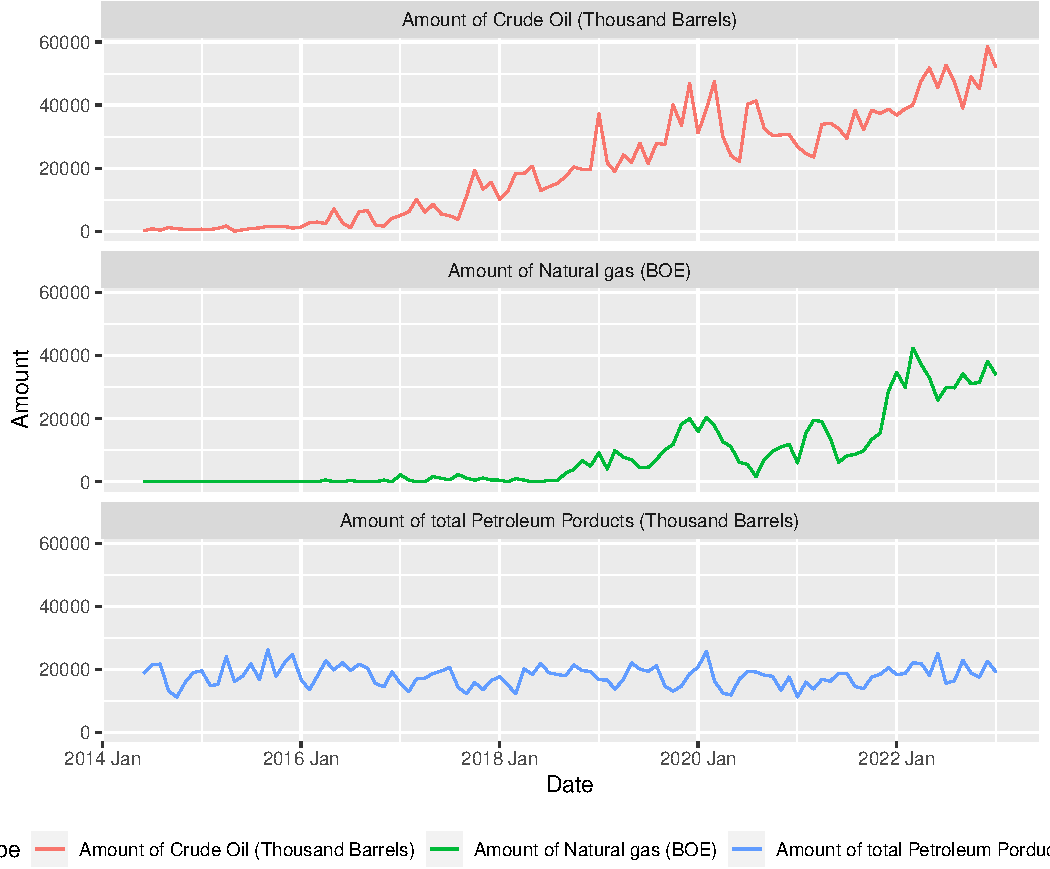
\includegraphics{draft1_files/figure-latex/overview by product-1} \end{center}

\hypertarget{time-series-patterns}{%
\paragraph{2.3 Time Series Patterns}\label{time-series-patterns}}

\begin{Shaded}
\begin{Highlighting}[]
\CommentTok{\# create seasonal plot of total exports monthly of Natural gas}
\NormalTok{total\_exp\_oecd }\SpecialCharTok{\%\textgreater{}\%} \FunctionTok{filter}\NormalTok{(}\StringTok{\textasciigrave{}}\AttributeTok{Export Type}\StringTok{\textasciigrave{}} \SpecialCharTok{==} \StringTok{"Amount of Natural gas (BOE)"}\NormalTok{) }\SpecialCharTok{\%\textgreater{}\%} 
  \FunctionTok{index\_by}\NormalTok{(Date) }\SpecialCharTok{\%\textgreater{}\%} 
  \FunctionTok{summarise}\NormalTok{(}\AttributeTok{Total\_Exports =} \FunctionTok{sum}\NormalTok{(}\StringTok{\textasciigrave{}}\AttributeTok{Amount}\StringTok{\textasciigrave{}}\NormalTok{)) }\SpecialCharTok{\%\textgreater{}\%} 
  \FunctionTok{gg\_season}\NormalTok{(Total\_Exports) }\SpecialCharTok{+}
  \FunctionTok{ylab}\NormalTok{(}\StringTok{"Total exports  of Natural Gas"}\NormalTok{) }\SpecialCharTok{+}
  \FunctionTok{ggtitle}\NormalTok{(}\StringTok{"Seasonal plot: US exports of natural gas to OECD"}\NormalTok{) }\SpecialCharTok{+}
  \FunctionTok{scale\_y\_continuous}\NormalTok{(}\AttributeTok{labels =} \FunctionTok{comma\_format}\NormalTok{())}
\end{Highlighting}
\end{Shaded}

\begin{center}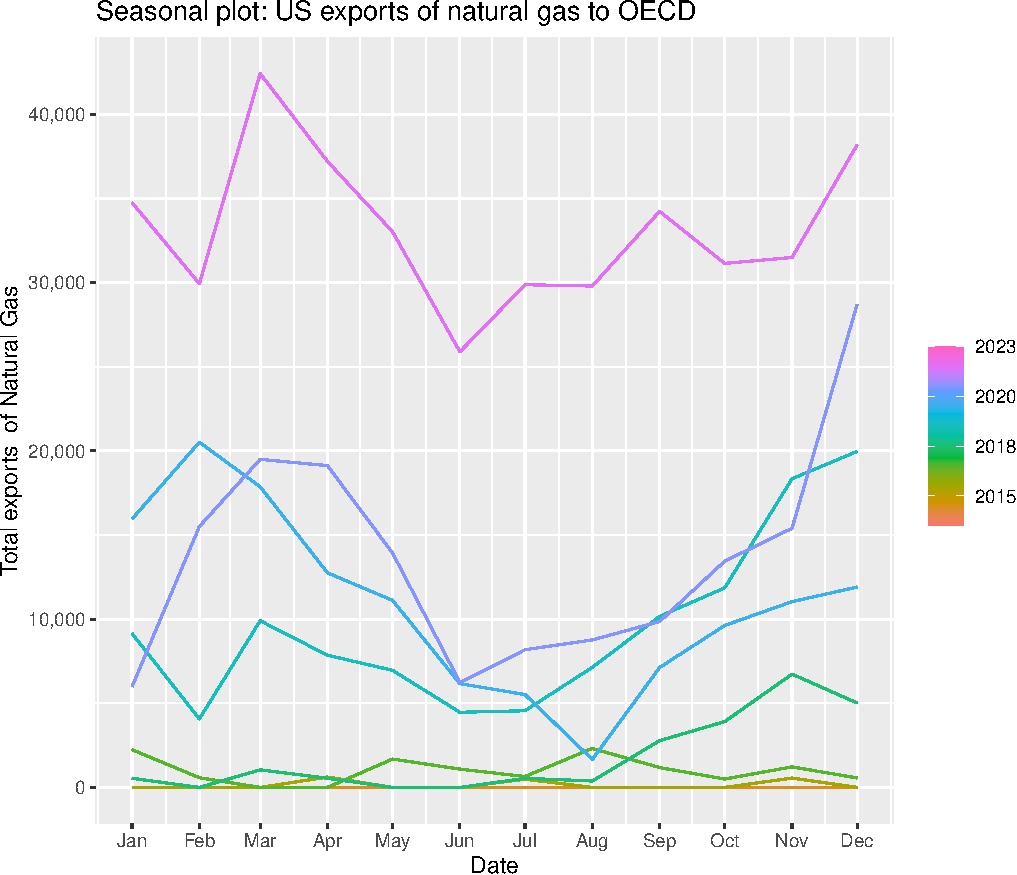
\includegraphics{draft1_files/figure-latex/Seasonal plot for each product-1} \end{center}

\begin{Shaded}
\begin{Highlighting}[]
\CommentTok{\# create seasonal plot of total exports monthly of Crude oil}
\NormalTok{total\_exp\_oecd }\SpecialCharTok{\%\textgreater{}\%} \FunctionTok{filter}\NormalTok{(}\StringTok{\textasciigrave{}}\AttributeTok{Export Type}\StringTok{\textasciigrave{}} \SpecialCharTok{==} \StringTok{"Amount of Crude Oil (Thousand Barrels)"}\NormalTok{) }\SpecialCharTok{\%\textgreater{}\%} 
  \FunctionTok{index\_by}\NormalTok{(Date) }\SpecialCharTok{\%\textgreater{}\%} 
  \FunctionTok{summarise}\NormalTok{(}\AttributeTok{Total\_Exports =} \FunctionTok{sum}\NormalTok{(}\StringTok{\textasciigrave{}}\AttributeTok{Amount}\StringTok{\textasciigrave{}}\NormalTok{)) }\SpecialCharTok{\%\textgreater{}\%} 
  \FunctionTok{gg\_season}\NormalTok{(Total\_Exports) }\SpecialCharTok{+}
  \FunctionTok{ylab}\NormalTok{(}\StringTok{"Total exports  of Crude oil"}\NormalTok{) }\SpecialCharTok{+}
  \FunctionTok{ggtitle}\NormalTok{(}\StringTok{"Seasonal plot: US exports of Crude Oil to OECD"}\NormalTok{) }\SpecialCharTok{+}
  \FunctionTok{scale\_y\_continuous}\NormalTok{(}\AttributeTok{labels =} \FunctionTok{comma\_format}\NormalTok{())}
\end{Highlighting}
\end{Shaded}

\begin{center}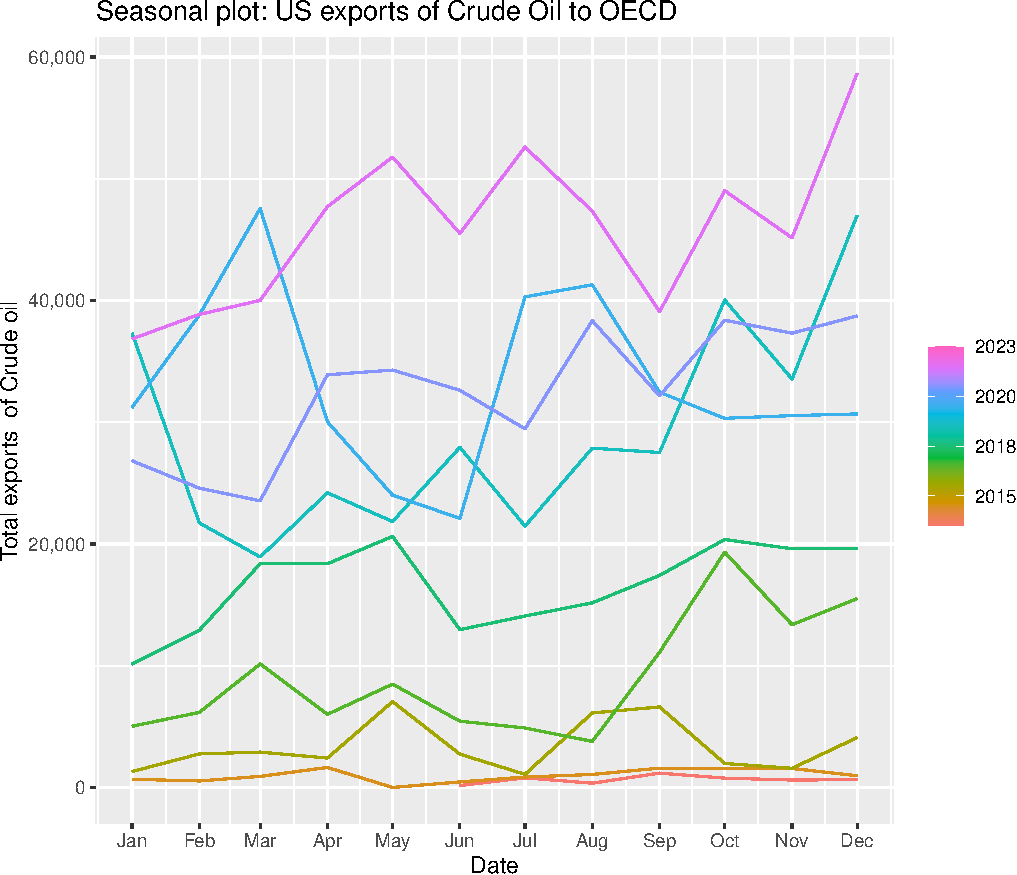
\includegraphics{draft1_files/figure-latex/Seasonal plot for each product-2} \end{center}

\begin{Shaded}
\begin{Highlighting}[]
\CommentTok{\# create seasonal plot of total exports monthly of Petroleum products}
\NormalTok{total\_exp\_oecd }\SpecialCharTok{\%\textgreater{}\%} \FunctionTok{filter}\NormalTok{(}\StringTok{\textasciigrave{}}\AttributeTok{Export Type}\StringTok{\textasciigrave{}} \SpecialCharTok{==} \StringTok{"Amount of total Petroleum Porducts (Thousand Barrels)"}\NormalTok{) }\SpecialCharTok{\%\textgreater{}\%} 
  \FunctionTok{index\_by}\NormalTok{(Date) }\SpecialCharTok{\%\textgreater{}\%} 
  \FunctionTok{summarise}\NormalTok{(}\AttributeTok{Total\_Exports =} \FunctionTok{sum}\NormalTok{(}\StringTok{\textasciigrave{}}\AttributeTok{Amount}\StringTok{\textasciigrave{}}\NormalTok{)) }\SpecialCharTok{\%\textgreater{}\%} 
  \FunctionTok{gg\_season}\NormalTok{(Total\_Exports) }\SpecialCharTok{+}
  \FunctionTok{ylab}\NormalTok{(}\StringTok{"Total exports  of Petroleum Products"}\NormalTok{) }\SpecialCharTok{+}
  \FunctionTok{ggtitle}\NormalTok{(}\StringTok{"Seasonal plot: US exports of Petroleum to OECD"}\NormalTok{) }\SpecialCharTok{+}
  \FunctionTok{scale\_y\_continuous}\NormalTok{(}\AttributeTok{labels =} \FunctionTok{comma\_format}\NormalTok{())}
\end{Highlighting}
\end{Shaded}

\begin{center}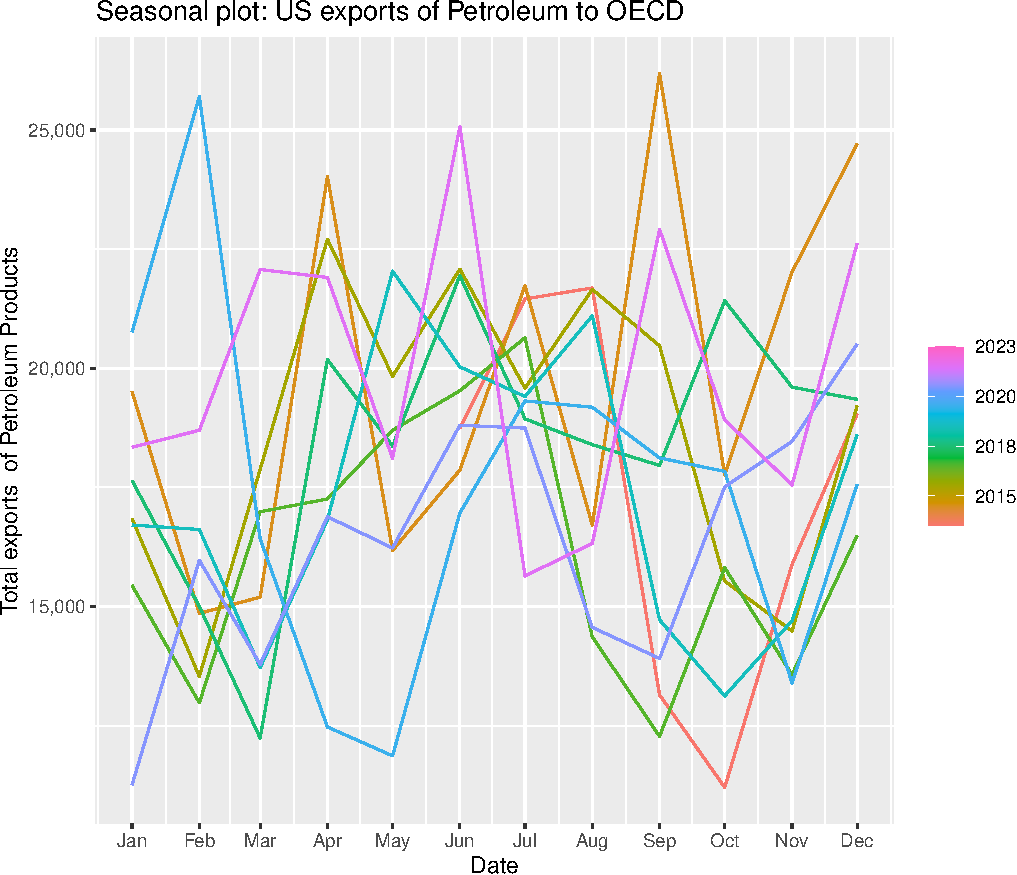
\includegraphics{draft1_files/figure-latex/Seasonal plot for each product-3} \end{center}

To further elaborate, the data analysis of US exports of oil products to
OECD shows that seasonal patterns can differ depending on the type of
product being exported. While natural gas and crude oil both display
some level of seasonality, petroleum products do not show any
significant trends.

In the case of natural gas, we can see a clear increase in exports
during the colder months, which could be due to increased demand for
heating purposes. Conversely, during the warmer months, exports tend to
decrease. This pattern is consistent throughout the years, with the
exception of some yearly fluctuations.

Regarding crude oil, the seasonal pattern is not as clear as with
natural gas. However, we still observe a similar trend where exports
tend to increase during the colder months and decrease during the warmer
months. Interestingly, we see a deviation from this pattern in 2022,
with exports remaining high even during spring and summer months. This
could be attributed to the political tensions caused by the Russian
invasion in Ukraine.

On the other hand, the export of petroleum products does not appear to
have any notable seasonal patterns. While there may be a slight increase
towards the end of each year, there is no clear trend observed
year-over-year.

Overall, analyzing seasonal patterns in the US export of oil products
can provide insights into demand patterns and other underlying factors
that affect the global oil market.

\begin{Shaded}
\begin{Highlighting}[]
\CommentTok{\#Subseries plots Natural gas}
\NormalTok{total\_exp\_oecd }\SpecialCharTok{\%\textgreater{}\%} \FunctionTok{filter}\NormalTok{(}\StringTok{\textasciigrave{}}\AttributeTok{Export Type}\StringTok{\textasciigrave{}} \SpecialCharTok{==} \StringTok{"Amount of Natural gas (BOE)"}\NormalTok{) }\SpecialCharTok{\%\textgreater{}\%} 
  \FunctionTok{index\_by}\NormalTok{(Date) }\SpecialCharTok{\%\textgreater{}\%} 
  \FunctionTok{summarise}\NormalTok{(}\AttributeTok{Total\_Exports =} \FunctionTok{sum}\NormalTok{(}\StringTok{\textasciigrave{}}\AttributeTok{Amount}\StringTok{\textasciigrave{}}\NormalTok{)) }\SpecialCharTok{\%\textgreater{}\%} 
  \FunctionTok{gg\_subseries}\NormalTok{(Total\_Exports) }\SpecialCharTok{+} 
  \FunctionTok{ylab}\NormalTok{(}\StringTok{"Total exports"}\NormalTok{) }\SpecialCharTok{+} 
  \FunctionTok{ggtitle}\NormalTok{(}\StringTok{"Subseries plot: US exports of natural gas"}\NormalTok{)}\SpecialCharTok{+}
  \FunctionTok{scale\_y\_continuous}\NormalTok{(}\AttributeTok{labels =} \FunctionTok{comma\_format}\NormalTok{())}
\end{Highlighting}
\end{Shaded}

\begin{center}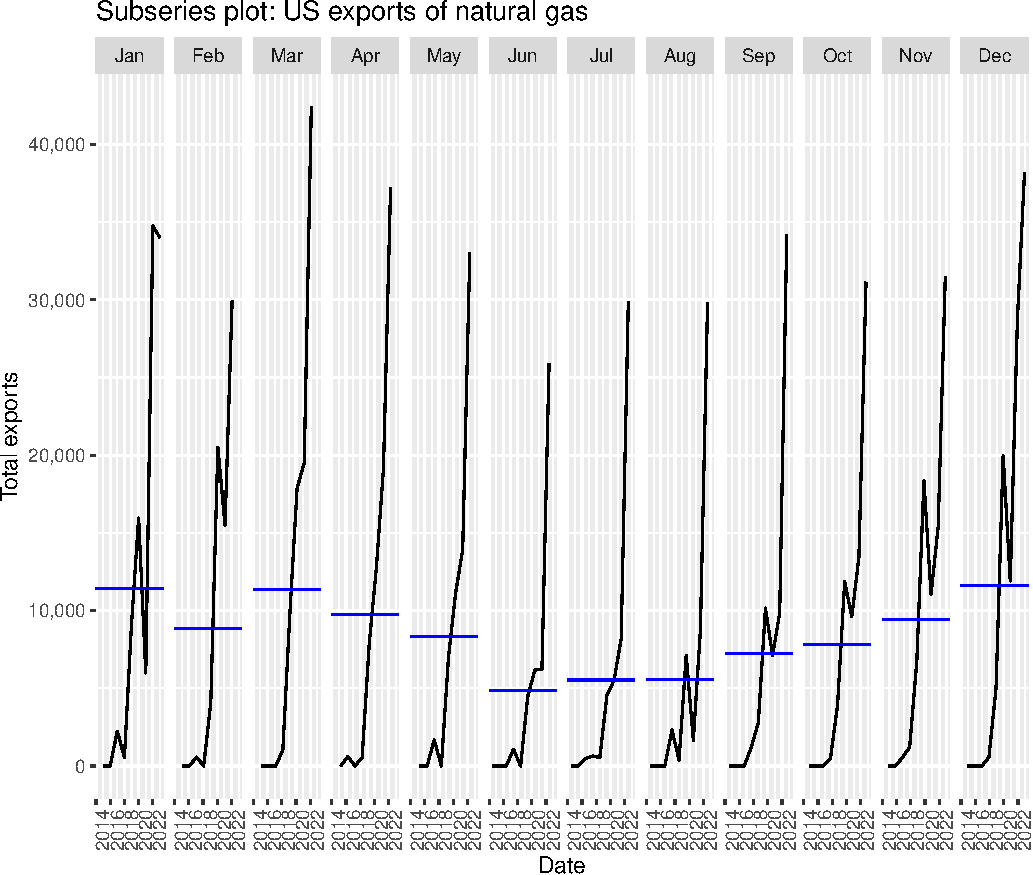
\includegraphics{draft1_files/figure-latex/seasonal-1} \end{center}

\begin{Shaded}
\begin{Highlighting}[]
\CommentTok{\#Subseries plots Crude oil}
\NormalTok{total\_exp\_oecd }\SpecialCharTok{\%\textgreater{}\%} \FunctionTok{filter}\NormalTok{(}\StringTok{\textasciigrave{}}\AttributeTok{Export Type}\StringTok{\textasciigrave{}} \SpecialCharTok{==} \StringTok{"Amount of Crude Oil (Thousand Barrels)"}\NormalTok{) }\SpecialCharTok{\%\textgreater{}\%} 
  \FunctionTok{index\_by}\NormalTok{(Date) }\SpecialCharTok{\%\textgreater{}\%} 
  \FunctionTok{summarise}\NormalTok{(}\AttributeTok{Total\_Exports =} \FunctionTok{sum}\NormalTok{(}\StringTok{\textasciigrave{}}\AttributeTok{Amount}\StringTok{\textasciigrave{}}\NormalTok{)) }\SpecialCharTok{\%\textgreater{}\%} 
  \FunctionTok{gg\_subseries}\NormalTok{(Total\_Exports) }\SpecialCharTok{+} 
  \FunctionTok{ylab}\NormalTok{(}\StringTok{"Total exports"}\NormalTok{) }\SpecialCharTok{+} 
  \FunctionTok{ggtitle}\NormalTok{(}\StringTok{"Subseries plot: US exports of Crude Oil"}\NormalTok{)}\SpecialCharTok{+}
  \FunctionTok{scale\_y\_continuous}\NormalTok{(}\AttributeTok{labels =} \FunctionTok{comma\_format}\NormalTok{())}
\end{Highlighting}
\end{Shaded}

\begin{center}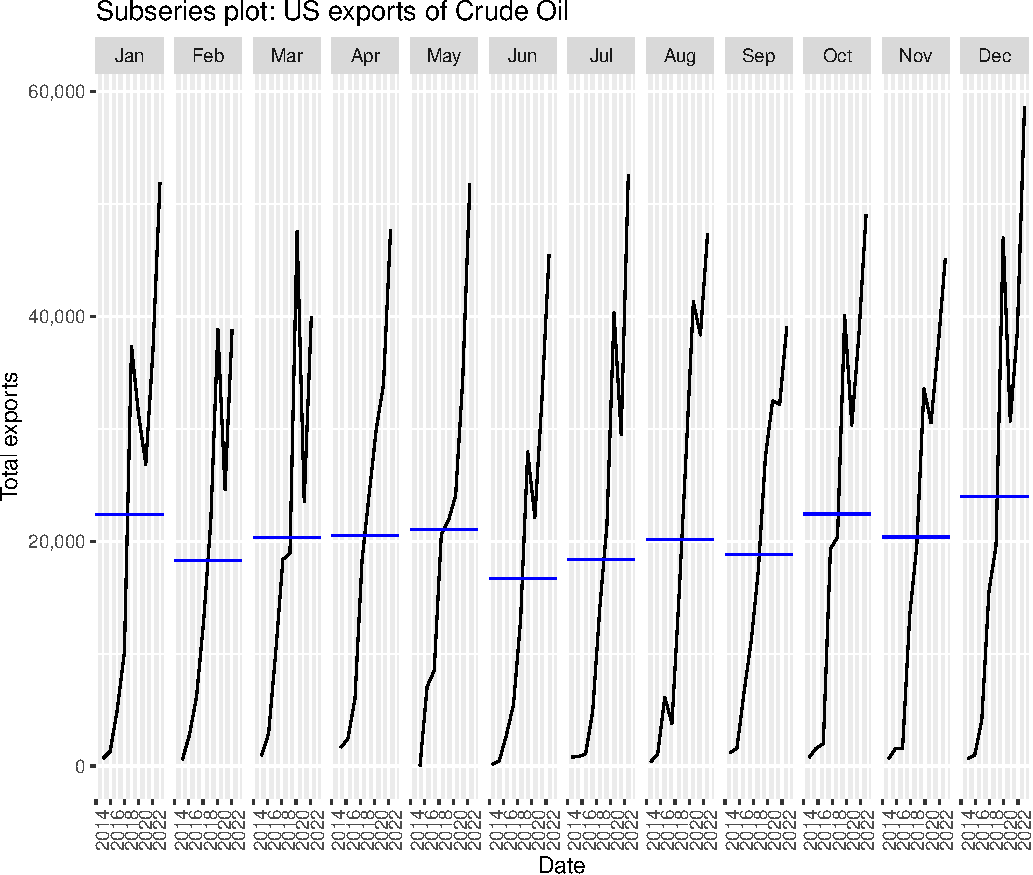
\includegraphics{draft1_files/figure-latex/seasonal-2} \end{center}

\begin{Shaded}
\begin{Highlighting}[]
\CommentTok{\#Subseries plots Petroleum products}
\NormalTok{total\_exp\_oecd }\SpecialCharTok{\%\textgreater{}\%} \FunctionTok{filter}\NormalTok{(}\StringTok{\textasciigrave{}}\AttributeTok{Export Type}\StringTok{\textasciigrave{}} \SpecialCharTok{==} \StringTok{"Amount of total Petroleum Porducts (Thousand Barrels)"}\NormalTok{) }\SpecialCharTok{\%\textgreater{}\%} 
  \FunctionTok{index\_by}\NormalTok{(Date) }\SpecialCharTok{\%\textgreater{}\%} 
  \FunctionTok{summarise}\NormalTok{(}\AttributeTok{Total\_Exports =} \FunctionTok{sum}\NormalTok{(}\StringTok{\textasciigrave{}}\AttributeTok{Amount}\StringTok{\textasciigrave{}}\NormalTok{)) }\SpecialCharTok{\%\textgreater{}\%} 
  \FunctionTok{gg\_subseries}\NormalTok{(Total\_Exports) }\SpecialCharTok{+} 
  \FunctionTok{ylab}\NormalTok{(}\StringTok{"Total exports"}\NormalTok{) }\SpecialCharTok{+} 
  \FunctionTok{ggtitle}\NormalTok{(}\StringTok{"Subseries plot: US exports of Petroleum Products"}\NormalTok{)}\SpecialCharTok{+}
  \FunctionTok{scale\_y\_continuous}\NormalTok{(}\AttributeTok{labels =} \FunctionTok{comma\_format}\NormalTok{())}
\end{Highlighting}
\end{Shaded}

\begin{center}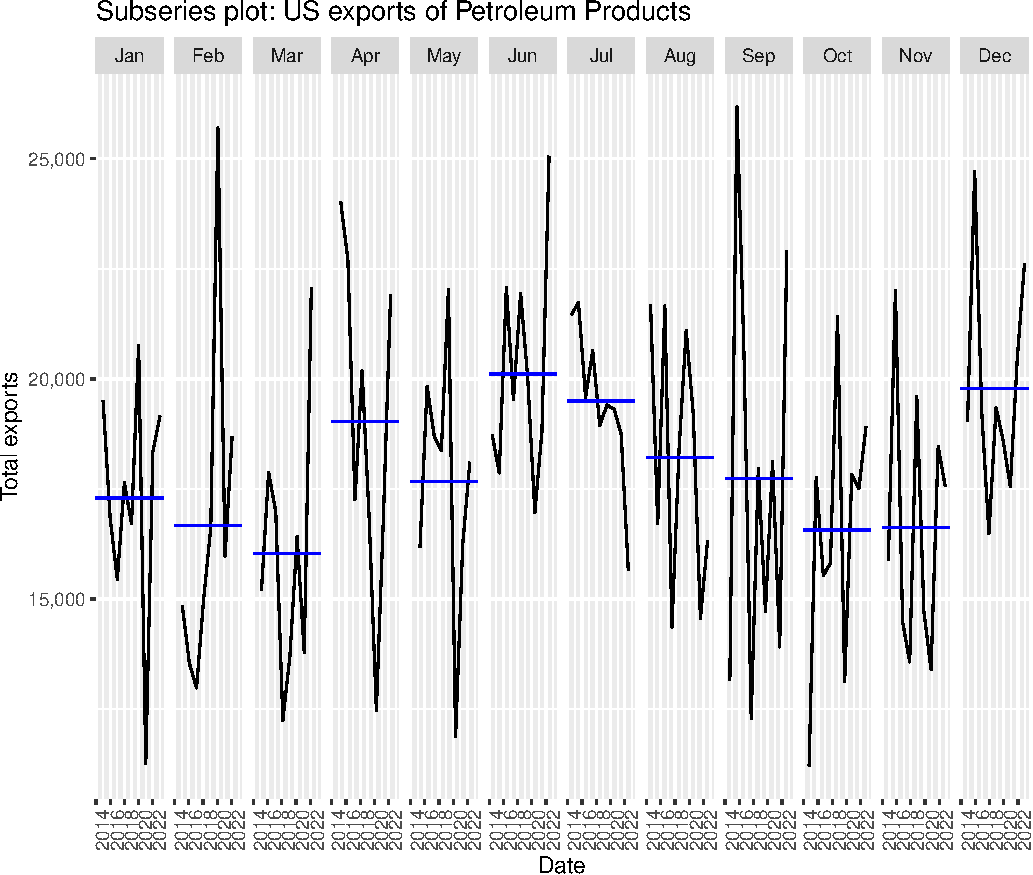
\includegraphics{draft1_files/figure-latex/seasonal-3} \end{center}

To gain a better understanding of seasonality, we created additional
plots known as subseries seasonal plots. These graphs provide a clearer
view of monthly exports and also display the means over each month for
the analyzed time series period.

When we look at the subseries seasonal plot for natural gas exports, we
can see a clear seasonality of increased natural gas exports during the
colder seasons, starting from September and decreasing in spring. From
the crude oil subseries seasonal plot, we can notice a huge increase in
December and January as well, indicating that these months have a strong
seasonal effect on crude oil exports. Finally, from the subseries
seasonal plot of Petroleum products, we can notice the same increase in
December, but there is a huge decrease in February and March. All other
months are fluctuating more randomly without displaying any clear
seasonality.

In general, the seasonal subseries plots for all three types of oil
exports to OECD reveal similar patterns to those seen in the seasonal
plots. There is a clear increase in exports during the colder seasons,
particularly in December and January, and a decrease during the warmer
seasons. However, there are some fluctuations and irregularities
throughout the year that do not follow a clear seasonal pattern.

\#\#\#\#2.4 ACF and White Noise

\begin{Shaded}
\begin{Highlighting}[]
\CommentTok{\#ACF plot without lag Natural Gas}

\NormalTok{total\_exp\_oecd }\SpecialCharTok{\%\textgreater{}\%} \FunctionTok{filter}\NormalTok{(}\StringTok{\textasciigrave{}}\AttributeTok{Export Type}\StringTok{\textasciigrave{}} \SpecialCharTok{==} \StringTok{"Amount of Natural gas (BOE)"}\NormalTok{) }\SpecialCharTok{\%\textgreater{}\%} 
  \FunctionTok{index\_by}\NormalTok{(Date) }\SpecialCharTok{\%\textgreater{}\%} 
  \FunctionTok{summarise}\NormalTok{(}\AttributeTok{Total\_Exports =} \FunctionTok{sum}\NormalTok{(}\StringTok{\textasciigrave{}}\AttributeTok{Amount}\StringTok{\textasciigrave{}}\NormalTok{)) }\SpecialCharTok{\%\textgreater{}\%} 
  \FunctionTok{ACF}\NormalTok{() }\SpecialCharTok{\%\textgreater{}\%}  \FunctionTok{autoplot}\NormalTok{()}
\end{Highlighting}
\end{Shaded}

\begin{center}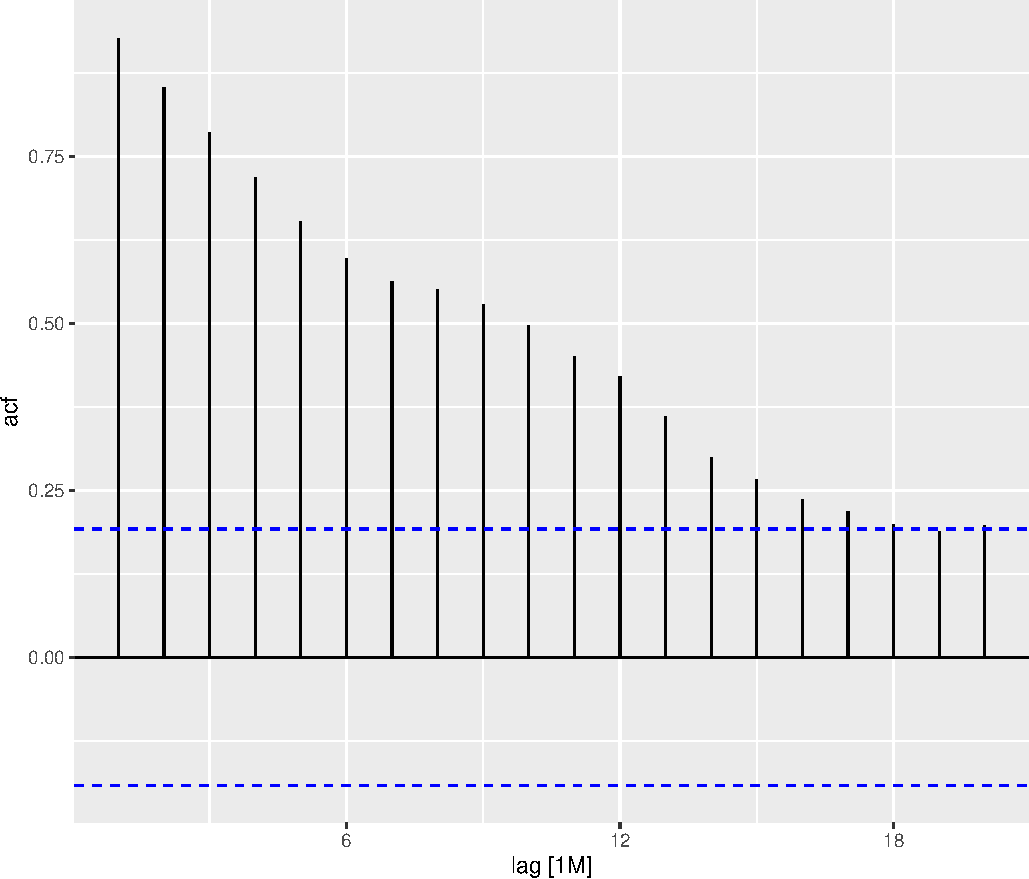
\includegraphics{draft1_files/figure-latex/Acf and white noise-1} \end{center}

\begin{Shaded}
\begin{Highlighting}[]
\CommentTok{\#ACF plot without lag Crude Oil}

\NormalTok{total\_exp\_oecd }\SpecialCharTok{\%\textgreater{}\%} \FunctionTok{filter}\NormalTok{(}\StringTok{\textasciigrave{}}\AttributeTok{Export Type}\StringTok{\textasciigrave{}} \SpecialCharTok{==} \StringTok{"Amount of Crude Oil (Thousand Barrels)"}\NormalTok{) }\SpecialCharTok{\%\textgreater{}\%} 
  \FunctionTok{index\_by}\NormalTok{(Date) }\SpecialCharTok{\%\textgreater{}\%} 
  \FunctionTok{summarise}\NormalTok{(}\AttributeTok{Total\_Exports =} \FunctionTok{sum}\NormalTok{(}\StringTok{\textasciigrave{}}\AttributeTok{Amount}\StringTok{\textasciigrave{}}\NormalTok{)) }\SpecialCharTok{\%\textgreater{}\%} 
  \FunctionTok{ACF}\NormalTok{() }\SpecialCharTok{\%\textgreater{}\%}  \FunctionTok{autoplot}\NormalTok{()}
\end{Highlighting}
\end{Shaded}

\begin{center}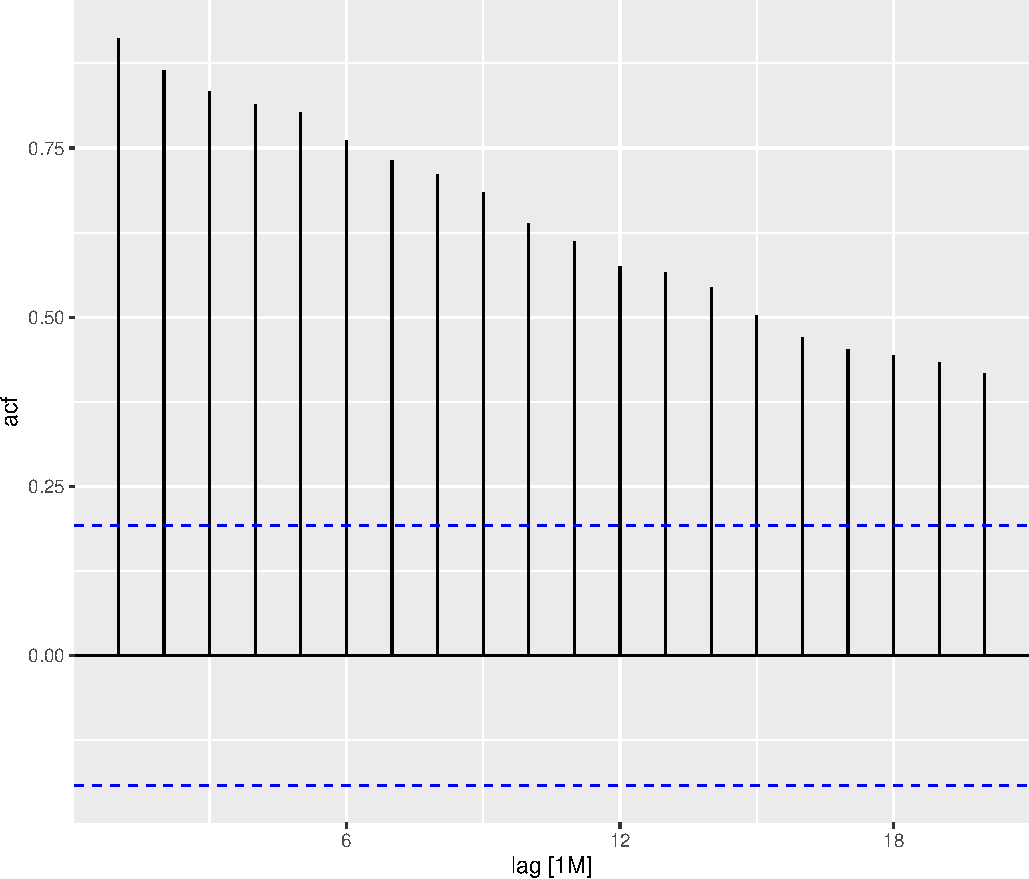
\includegraphics{draft1_files/figure-latex/Acf and white noise-2} \end{center}

\begin{Shaded}
\begin{Highlighting}[]
\CommentTok{\#ACF plot without lag Petroleum}

\NormalTok{total\_exp\_oecd }\SpecialCharTok{\%\textgreater{}\%} \FunctionTok{filter}\NormalTok{(}\StringTok{\textasciigrave{}}\AttributeTok{Export Type}\StringTok{\textasciigrave{}} \SpecialCharTok{==} \StringTok{"Amount of total Petroleum Porducts (Thousand Barrels)"}\NormalTok{) }\SpecialCharTok{\%\textgreater{}\%} 
  \FunctionTok{index\_by}\NormalTok{(Date) }\SpecialCharTok{\%\textgreater{}\%} 
  \FunctionTok{summarise}\NormalTok{(}\AttributeTok{Total\_Exports =} \FunctionTok{sum}\NormalTok{(}\StringTok{\textasciigrave{}}\AttributeTok{Amount}\StringTok{\textasciigrave{}}\NormalTok{)) }\SpecialCharTok{\%\textgreater{}\%} 
  \FunctionTok{ACF}\NormalTok{() }\SpecialCharTok{\%\textgreater{}\%}  \FunctionTok{autoplot}\NormalTok{()}
\end{Highlighting}
\end{Shaded}

\begin{center}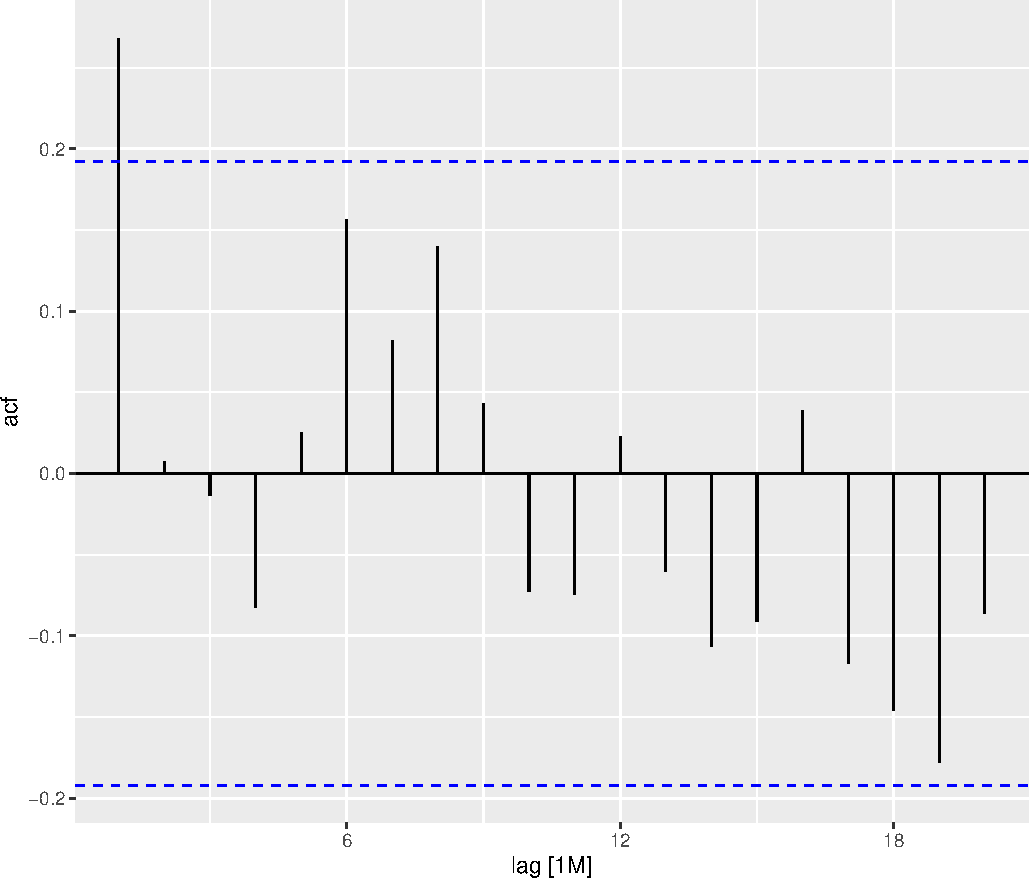
\includegraphics{draft1_files/figure-latex/Acf and white noise-3} \end{center}

The autocorrelation function (ACF) plot displays the correlation between
a time series and its own lagged values. A high ACF value for a
particular lag indicates that the current values of the time series are
significantly correlated with the past values at that lag.

The ACF plots for US exports of Natural Gas, Crude Oil to OECD reveal
interesting insights regarding the seasonality and trends in the time
series. In the case of Natural Gas and Crude Oil, the ACF plots
demonstrate a significant positive correlation, indicating the presence
of high trend component with slight seasonality patterns observed as.
However, these plots reflect a dominant upward trend, as evidenced by
the substantial increase in exports. The trend component seems to be
overtaking the seasonality, suggesting that the overall upward trend in
exports is more prominent than the periodic variation in the data.

The ACF plot for US exports of Petroleum Products to OECD indicates that
there is no noticeable seasonality in the time series. The first three
lags show significant positive correlations, suggesting some short-term
dependence between current exports and those from 1 to 3 months ago.
However, beyond the third lag, the ACF values fall within the confidence
interval, indicating a weakening of the correlation. This suggests that
there is no clear and consistent pattern of seasonality in the exports
of petroleum products.

Finally, based on the ACF plots of the US exports of natural gas, crude
oil, and petroleum products to OECD, we can conclude that the time
series do not appear to be white noise.

\hypertarget{time-series-decomposition}{%
\subsubsection{3. Time series
decomposition}\label{time-series-decomposition}}

\hypertarget{adjustments}{%
\paragraph{3.1. Adjustments}\label{adjustments}}

After a thorough review of the data, we determined that no adjustments
were necessary. We did not observe any calendar or population effects on
the monthly exports data, and the exports data is already presented in
barrels or barrels of oil equivalent (BOE), so no inflation adjustments
were required.

\hypertarget{transformations}{%
\paragraph{3.2. Transformations}\label{transformations}}

Given the nature of the three data sets that are being used: Crude Oil
Exports, Petroleum exports and Natural gas exports we decided that
certain transformations might be necessary for further analysis. Not
normal distribution of the data and differing variance were seen as
potential threat for correct conclusions. We identified Box-Cox
transformation as necessary to continue since it stabilizes the variance
of the data and makes the distribution more normal. This will improve
the reliability of the statistical tests and provide more accurate
results.

For Box-Cox transformation to be performed we found lambda for each time
series and than use it to transform the time series.

\begin{Shaded}
\begin{Highlighting}[]
\NormalTok{lambda1 }\OtherTok{\textless{}{-}}\NormalTok{ total\_exp\_oecd }\SpecialCharTok{\%\textgreater{}\%} 
  \FunctionTok{filter}\NormalTok{(}\StringTok{\textasciigrave{}}\AttributeTok{Export Type}\StringTok{\textasciigrave{}} \SpecialCharTok{==} \StringTok{"Amount of Crude Oil (Thousand Barrels)"}\NormalTok{) }\SpecialCharTok{\%\textgreater{}\%} 
  \FunctionTok{index\_by}\NormalTok{(Date) }\SpecialCharTok{\%\textgreater{}\%} 
  \FunctionTok{summarise}\NormalTok{(}\AttributeTok{Total\_Exports =} \FunctionTok{sum}\NormalTok{(Amount)) }\SpecialCharTok{\%\textgreater{}\%} 
  \FunctionTok{features}\NormalTok{(Total\_Exports, }\AttributeTok{features =}\NormalTok{ guerrero) }\SpecialCharTok{\%\textgreater{}\%} 
  \FunctionTok{pull}\NormalTok{(lambda\_guerrero)}

\NormalTok{crude\_oil\_bx }\OtherTok{\textless{}{-}}\NormalTok{total\_exp\_oecd }\SpecialCharTok{\%\textgreater{}\%} 
  \FunctionTok{filter}\NormalTok{(}\StringTok{\textasciigrave{}}\AttributeTok{Export Type}\StringTok{\textasciigrave{}} \SpecialCharTok{==} \StringTok{"Amount of Crude Oil (Thousand Barrels)"}\NormalTok{) }\SpecialCharTok{\%\textgreater{}\%} 
  \FunctionTok{index\_by}\NormalTok{(Date) }\SpecialCharTok{\%\textgreater{}\%} 
  \FunctionTok{summarise}\NormalTok{(}\AttributeTok{Total\_Exports =} \FunctionTok{sum}\NormalTok{(Amount)) }\SpecialCharTok{\%\textgreater{}\%} 
  \FunctionTok{mutate}\NormalTok{(}\AttributeTok{Total\_Exports =} \FunctionTok{box\_cox}\NormalTok{(Total\_Exports }\SpecialCharTok{+} \DecValTok{1}\NormalTok{, lambda1))}

\NormalTok{crude\_oil\_bx}
\end{Highlighting}
\end{Shaded}

\begin{verbatim}
## # A tsibble: 104 x 2 [1M]
##        Date Total_Exports
##       <mth>         <dbl>
##  1 2014 Jun          13.9
##  2 2014 Jul          26.7
##  3 2014 Aug          19.3
##  4 2014 Sep          31.2
##  5 2014 Oct          26.4
##  6 2014 Nov          24.1
##  7 2014 Dec          24.5
##  8 2015 Jan          25.0
##  9 2015 Feb          22.9
## 10 2015 Mar          28.2
## # ... with 94 more rows
\end{verbatim}

\begin{Shaded}
\begin{Highlighting}[]
\NormalTok{lambda2 }\OtherTok{\textless{}{-}}\NormalTok{ total\_exp\_oecd }\SpecialCharTok{\%\textgreater{}\%} 
  \FunctionTok{filter}\NormalTok{(}\StringTok{\textasciigrave{}}\AttributeTok{Export Type}\StringTok{\textasciigrave{}} \SpecialCharTok{==} \StringTok{"Amount of total Petroleum Porducts (Thousand Barrels)"}\NormalTok{) }\SpecialCharTok{\%\textgreater{}\%} 
  \FunctionTok{index\_by}\NormalTok{(Date) }\SpecialCharTok{\%\textgreater{}\%} 
  \FunctionTok{summarise}\NormalTok{(}\AttributeTok{Total\_Exports =} \FunctionTok{sum}\NormalTok{(Amount)) }\SpecialCharTok{\%\textgreater{}\%} 
  \FunctionTok{features}\NormalTok{(Total\_Exports, }\AttributeTok{features =}\NormalTok{ guerrero) }\SpecialCharTok{\%\textgreater{}\%} 
  \FunctionTok{pull}\NormalTok{(lambda\_guerrero)}

\NormalTok{pet\_prod\_bx }\OtherTok{\textless{}{-}}\NormalTok{total\_exp\_oecd }\SpecialCharTok{\%\textgreater{}\%} 
  \FunctionTok{filter}\NormalTok{(}\StringTok{\textasciigrave{}}\AttributeTok{Export Type}\StringTok{\textasciigrave{}} \SpecialCharTok{==} \StringTok{"Amount of total Petroleum Porducts (Thousand Barrels)"}\NormalTok{) }\SpecialCharTok{\%\textgreater{}\%} 
  \FunctionTok{index\_by}\NormalTok{(Date) }\SpecialCharTok{\%\textgreater{}\%} 
  \FunctionTok{summarise}\NormalTok{(}\AttributeTok{Total\_Exports =} \FunctionTok{sum}\NormalTok{(Amount)) }\SpecialCharTok{\%\textgreater{}\%} 
  \FunctionTok{mutate}\NormalTok{(}\AttributeTok{Total\_Exports =} \FunctionTok{box\_cox}\NormalTok{(Total\_Exports }\SpecialCharTok{+} \DecValTok{1}\NormalTok{, lambda2))}

\NormalTok{lambda3 }\OtherTok{\textless{}{-}}\NormalTok{ total\_exp\_oecd }\SpecialCharTok{\%\textgreater{}\%} 
  \FunctionTok{filter}\NormalTok{(}\StringTok{\textasciigrave{}}\AttributeTok{Export Type}\StringTok{\textasciigrave{}} \SpecialCharTok{==} \StringTok{"Amount of Natural gas (BOE)"}\NormalTok{) }\SpecialCharTok{\%\textgreater{}\%} 
  \FunctionTok{index\_by}\NormalTok{(Date) }\SpecialCharTok{\%\textgreater{}\%} 
  \FunctionTok{summarise}\NormalTok{(}\AttributeTok{Total\_Exports =} \FunctionTok{sum}\NormalTok{(Amount)) }\SpecialCharTok{\%\textgreater{}\%} 
  \FunctionTok{features}\NormalTok{(Total\_Exports, }\AttributeTok{features =}\NormalTok{ guerrero) }\SpecialCharTok{\%\textgreater{}\%} 
  \FunctionTok{pull}\NormalTok{(lambda\_guerrero)}

\NormalTok{nat\_gas\_bx }\OtherTok{\textless{}{-}}\NormalTok{total\_exp\_oecd }\SpecialCharTok{\%\textgreater{}\%} 
  \FunctionTok{filter}\NormalTok{(}\StringTok{\textasciigrave{}}\AttributeTok{Export Type}\StringTok{\textasciigrave{}} \SpecialCharTok{==} \StringTok{"Amount of Natural gas (BOE)"}\NormalTok{) }\SpecialCharTok{\%\textgreater{}\%} 
  \FunctionTok{index\_by}\NormalTok{(Date) }\SpecialCharTok{\%\textgreater{}\%} 
  \FunctionTok{summarise}\NormalTok{(}\AttributeTok{Total\_Exports =} \FunctionTok{sum}\NormalTok{(Amount)) }\SpecialCharTok{\%\textgreater{}\%} 
  \FunctionTok{mutate}\NormalTok{(}\AttributeTok{Total\_Exports =} \FunctionTok{box\_cox}\NormalTok{(Total\_Exports }\SpecialCharTok{+} \DecValTok{1}\NormalTok{, lambda3))}

\NormalTok{nat\_gas\_bx }\OtherTok{\textless{}{-}} \FunctionTok{filter}\NormalTok{(nat\_gas\_bx, Date }\SpecialCharTok{\textgreater{}=} \FunctionTok{as.Date}\NormalTok{(}\StringTok{"2016{-}01{-}01"}\NormalTok{))}
\end{Highlighting}
\end{Shaded}

\hypertarget{decomposition}{%
\paragraph{3.3. Decomposition}\label{decomposition}}

\#\#\#STL Decomposition

\begin{Shaded}
\begin{Highlighting}[]
\NormalTok{dcmp\_crude\_oil }\OtherTok{\textless{}{-}}\NormalTok{ crude\_oil\_bx }\SpecialCharTok{\%\textgreater{}\%}
  \FunctionTok{model}\NormalTok{(}\AttributeTok{stl =} \FunctionTok{STL}\NormalTok{(Total\_Exports))}

\FunctionTok{components}\NormalTok{(dcmp\_crude\_oil)}
\end{Highlighting}
\end{Shaded}

\begin{verbatim}
## # A dable: 104 x 7 [1M]
## # Key:     .model [1]
## # :        Total_Exports = trend + season_year + remainder
##    .model     Date Total_Exports trend season_year remainder season_adjust
##    <chr>     <mth>         <dbl> <dbl>       <dbl>     <dbl>         <dbl>
##  1 stl    2014 Jun          13.9  24.0      -5.85     -4.28           19.7
##  2 stl    2014 Jul          26.7  24.1      -5.38      8.00           32.1
##  3 stl    2014 Aug          19.3  24.1      -1.83     -2.96           21.2
##  4 stl    2014 Sep          31.2  24.2       3.74      3.24           27.4
##  5 stl    2014 Oct          26.4  24.3       2.83     -0.785          23.5
##  6 stl    2014 Nov          24.1  24.4      -1.81      1.52           26.0
##  7 stl    2014 Dec          24.5  24.6       0.841    -0.900          23.7
##  8 stl    2015 Jan          25.0  24.8       0.374    -0.118          24.7
##  9 stl    2015 Feb          22.9  25.0       0.775    -2.87           22.1
## 10 stl    2015 Mar          28.2  25.2       4.84     -1.86           23.3
## # ... with 94 more rows
\end{verbatim}

\begin{Shaded}
\begin{Highlighting}[]
\NormalTok{dcmp\_oil\_prod }\OtherTok{\textless{}{-}}\NormalTok{ pet\_prod\_bx }\SpecialCharTok{\%\textgreater{}\%}
  \FunctionTok{model}\NormalTok{(}\AttributeTok{stl =} \FunctionTok{STL}\NormalTok{(Total\_Exports))}

\FunctionTok{components}\NormalTok{(dcmp\_oil\_prod)}
\end{Highlighting}
\end{Shaded}

\begin{verbatim}
## # A dable: 104 x 7 [1M]
## # Key:     .model [1]
## # :        Total_Exports = trend + season_year + remainder
##    .model     Date Total_Exports trend season_year remainder season_adjust
##    <chr>     <mth>         <dbl> <dbl>       <dbl>     <dbl>         <dbl>
##  1 stl    2014 Jun          548.  508.       35.4       4.41          513.
##  2 stl    2014 Jul          594.  511.       44.4      38.1           549.
##  3 stl    2014 Aug          597.  514.       17.6      65.9           580.
##  4 stl    2014 Sep          445.  517.       -5.36    -66.5           450.
##  5 stl    2014 Oct          405.  520.      -34.6     -80.1           439.
##  6 stl    2014 Nov          497.  522.      -22.0      -3.25          519.
##  7 stl    2014 Dec          553.  525.       30.6      -2.55          523.
##  8 stl    2015 Jan          561.  529.      -10.2      43.0           572.
##  9 stl    2015 Feb          478.  532.      -44.7      -8.88          523.
## 10 stl    2015 Mar          485.  535.      -44.0      -6.38          528.
## # ... with 94 more rows
\end{verbatim}

\begin{Shaded}
\begin{Highlighting}[]
\NormalTok{dcmp\_nat\_gas }\OtherTok{\textless{}{-}}\NormalTok{ nat\_gas\_bx }\SpecialCharTok{\%\textgreater{}\%}
  \FunctionTok{model}\NormalTok{(}\AttributeTok{stl =} \FunctionTok{STL}\NormalTok{(Total\_Exports))}

\FunctionTok{components}\NormalTok{(dcmp\_nat\_gas)}
\end{Highlighting}
\end{Shaded}

\begin{verbatim}
## # A dable: 85 x 7 [1M]
## # Key:     .model [1]
## # :        Total_Exports = trend + season_year + remainder
##    .model     Date Total_Exports trend season_year remainder season_adjust
##    <chr>     <mth>         <dbl> <dbl>       <dbl>     <dbl>         <dbl>
##  1 stl    2016 Jan           0    1.43      10.3     -11.7         -10.3  
##  2 stl    2016 Feb           0    2.72      -0.425    -2.30          0.425
##  3 stl    2016 Mar           0    4.02       4.69     -8.71         -4.69 
##  4 stl    2016 Apr          28.9  5.31       3.60     20.0          25.3  
##  5 stl    2016 May           0    6.60      -3.05     -3.56          3.05 
##  6 stl    2016 Jun           0    7.90     -13.8       5.88         13.8  
##  7 stl    2016 Jul          26.2  9.20      -5.88     22.8          32.0  
##  8 stl    2016 Aug           0   10.6      -10.7       0.105        10.7  
##  9 stl    2016 Sep           0   11.9       -1.78    -10.2           1.78 
## 10 stl    2016 Oct           0   13.3       -1.16    -12.2           1.16 
## # ... with 75 more rows
\end{verbatim}

\begin{Shaded}
\begin{Highlighting}[]
\FunctionTok{components}\NormalTok{(dcmp\_crude\_oil) }\SpecialCharTok{\%\textgreater{}\%} \FunctionTok{autoplot}\NormalTok{()}
\end{Highlighting}
\end{Shaded}

\begin{center}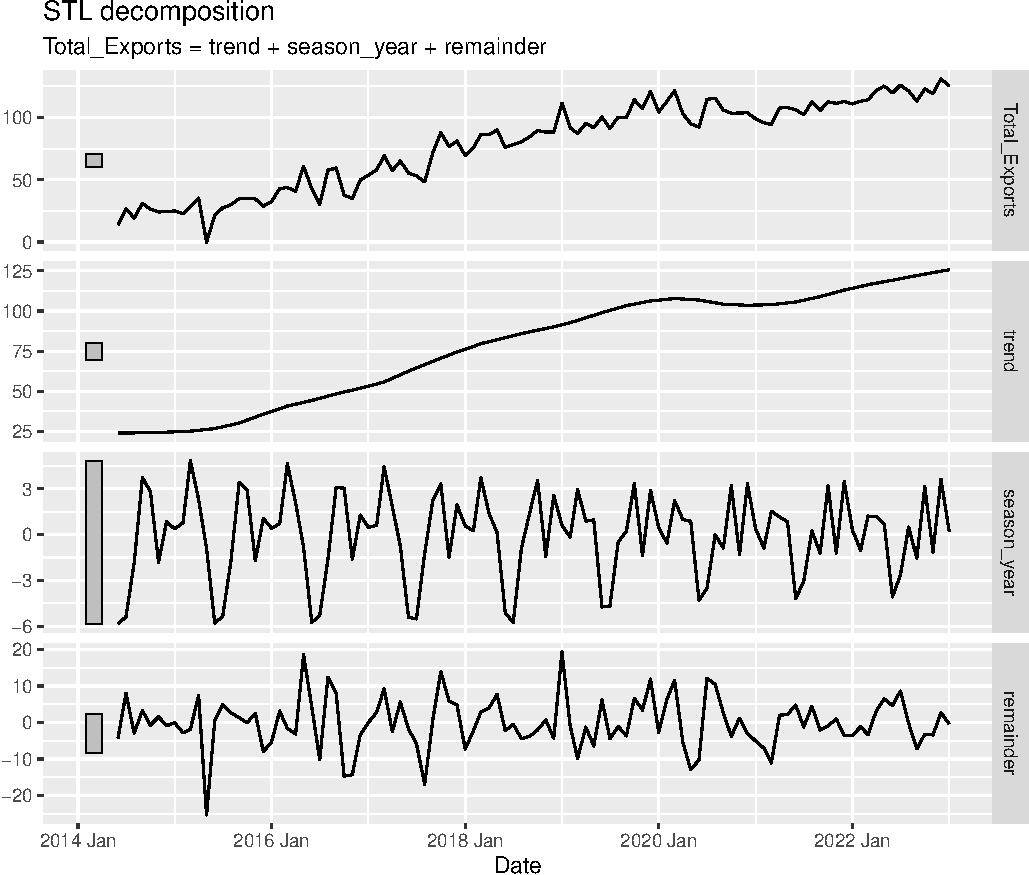
\includegraphics{draft1_files/figure-latex/Plotting components-1} \end{center}

\begin{Shaded}
\begin{Highlighting}[]
\FunctionTok{components}\NormalTok{(dcmp\_oil\_prod) }\SpecialCharTok{\%\textgreater{}\%} \FunctionTok{autoplot}\NormalTok{()}
\end{Highlighting}
\end{Shaded}

\begin{center}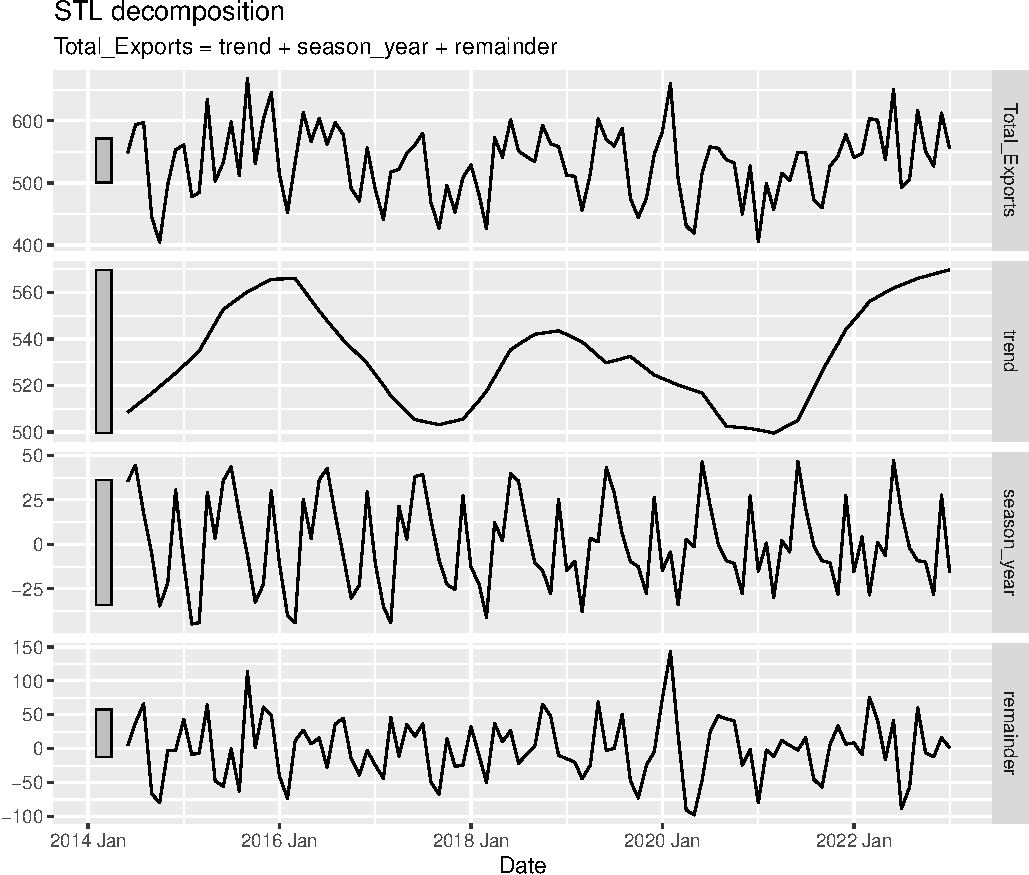
\includegraphics{draft1_files/figure-latex/Plotting components-2} \end{center}

\begin{Shaded}
\begin{Highlighting}[]
\FunctionTok{components}\NormalTok{(dcmp\_nat\_gas) }\SpecialCharTok{\%\textgreater{}\%} \FunctionTok{autoplot}\NormalTok{()}
\end{Highlighting}
\end{Shaded}

\begin{center}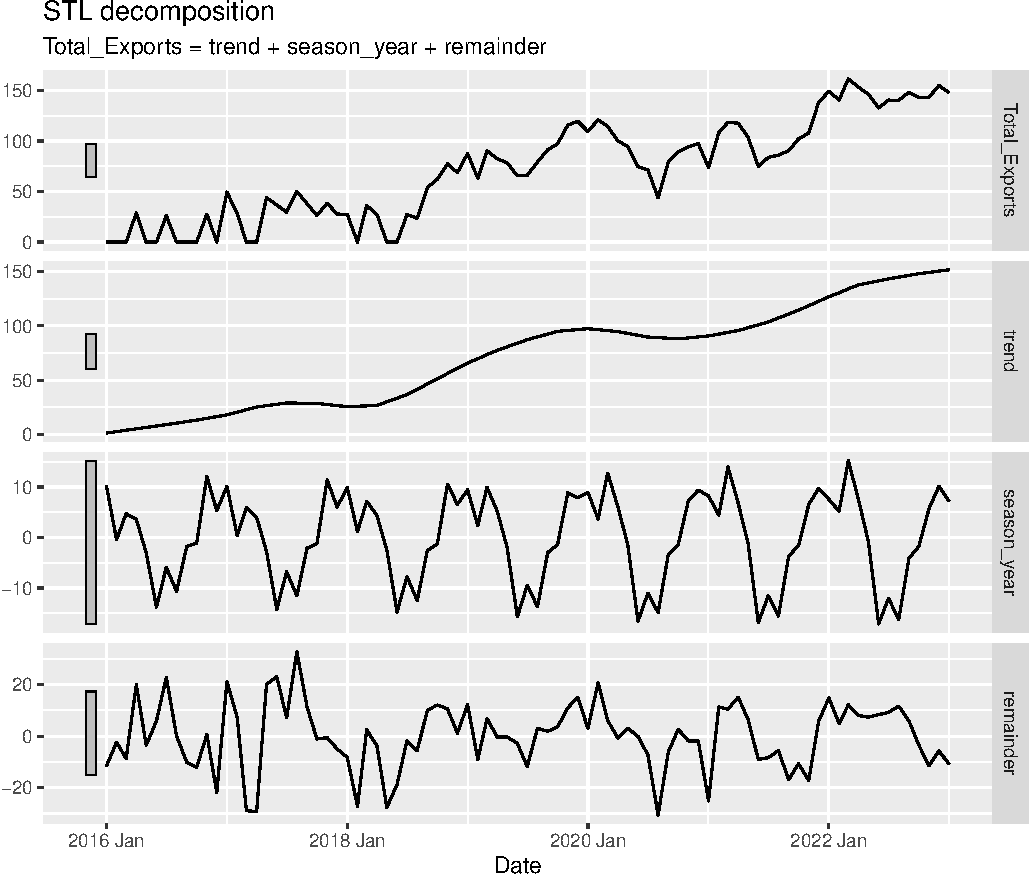
\includegraphics{draft1_files/figure-latex/Plotting components-3} \end{center}

We used STL decomposition to decompose the Box-Cox transformed time
series into three components: trend, seasonal, and residual. Four graphs
were plotted, three of which display the trend, seasonal, and residual
components, respectively while fourth one, the one at the top, represent
the export amounts from 2013 to 2023.

Looking at the graphs we see that in case of natural gas exports actual
patterns can only be seen appearing after approximately 2016 when the
U.S.

There are several conclusions to be drawn looking at the STL
decomposition. First of all, we can see clear trend in exports of crude
oil and natural gas while petroleum products does not have clear trend.
In both cases of exports of crude oil and natural gas we can clearly see
slight drops in exports after 2020 which can be explained by COVID 19
pandemic and continued growths after situation normalized. Another
observation worth mentioning is the fact that exports of two mentioned
products hits all time high around the year 2022. This can be explained
by huge declines of both products from Russia after sanction were
imposed.

Moreover, we can see seasonality in exports of all three products.That
is no surprise, given that all energy products are highly reactive to
different seasons.

After decomposing the data of all three time series and looking at each
components separately we decided that exports of petroleum products will
not be analysed further. Exports of petroleum products to OECD Europe
markets does not have clear trend therefore indicating that Russian
invasion in Ukraine did not have positive effect on growing imports from
US. This can be explained by the fact that embargo on refined oil
products from EU 27 was introduced as of 5 February 2023. Therefore,
Russian war on Ukraine and sanctions on Russia that followed did not
have any visible effect on US exports of petroleum products to OECD
Europe markets.

\hypertarget{the-forecasters-toolbox}{%
\subsection{4. The forecaster's toolbox}\label{the-forecasters-toolbox}}

\hypertarget{finding-the-fit}{%
\paragraph{4.1. Finding the fit}\label{finding-the-fit}}

When choosing from four possible simple forecasting methods the
intuition tells us that the most appropriate method in our case is Drift
method. Clear trend is seen in both crude oil and natural gas exports
data and drift method allows the forecasts to increase or decrease over
time based on the change in the historical data.

\begin{Shaded}
\begin{Highlighting}[]
\NormalTok{crude\_oil\_tr }\OtherTok{\textless{}{-}}\NormalTok{ crude\_oil\_bx }\SpecialCharTok{\%\textgreater{}\%} 
  \FunctionTok{filter}\NormalTok{(Date }\SpecialCharTok{\textgreater{}=} \FunctionTok{as.Date}\NormalTok{(}\StringTok{"2010{-}06{-}01"}\NormalTok{), Date }\SpecialCharTok{\textless{}=} \FunctionTok{as.Date}\NormalTok{(}\StringTok{"2020{-}06{-}01"}\NormalTok{))}

\NormalTok{crude\_oil\_fit }\OtherTok{\textless{}{-}}\NormalTok{ crude\_oil\_tr }\SpecialCharTok{\%\textgreater{}\%} 
  \FunctionTok{model}\NormalTok{(}
    \AttributeTok{Mean =} \FunctionTok{MEAN}\NormalTok{(Total\_Exports),}
    \AttributeTok{Naive =} \FunctionTok{NAIVE}\NormalTok{(Total\_Exports),}
    \AttributeTok{SNaive =} \FunctionTok{SNAIVE}\NormalTok{(Total\_Exports),}
    \AttributeTok{Drift =} \FunctionTok{RW}\NormalTok{(Total\_Exports }\SpecialCharTok{\textasciitilde{}} \FunctionTok{drift}\NormalTok{())}
\NormalTok{  )}

\NormalTok{crude\_oil\_fc }\OtherTok{\textless{}{-}}\NormalTok{ crude\_oil\_fit }\SpecialCharTok{\%\textgreater{}\%} 
  \FunctionTok{forecast}\NormalTok{(}\AttributeTok{h =} \DecValTok{36}\NormalTok{)}

\NormalTok{crude\_oil\_fc }\SpecialCharTok{\%\textgreater{}\%} 
  \FunctionTok{autoplot}\NormalTok{(}
\NormalTok{    crude\_oil\_bx,}
    \AttributeTok{level =} \ConstantTok{NULL}
\NormalTok{  ) }\SpecialCharTok{+}
  \FunctionTok{labs}\NormalTok{(}
    \AttributeTok{y =} \StringTok{"Thousand Barrels"}\NormalTok{,}
    \AttributeTok{title =} \StringTok{"Forecasts for U.S. Crude Oil exports to OECD Europe"}
\NormalTok{  ) }\SpecialCharTok{+}
  \FunctionTok{guides}\NormalTok{(}\AttributeTok{colour =} \FunctionTok{guide\_legend}\NormalTok{(}\AttributeTok{title =} \StringTok{"Forecast"}\NormalTok{))}
\end{Highlighting}
\end{Shaded}

\begin{center}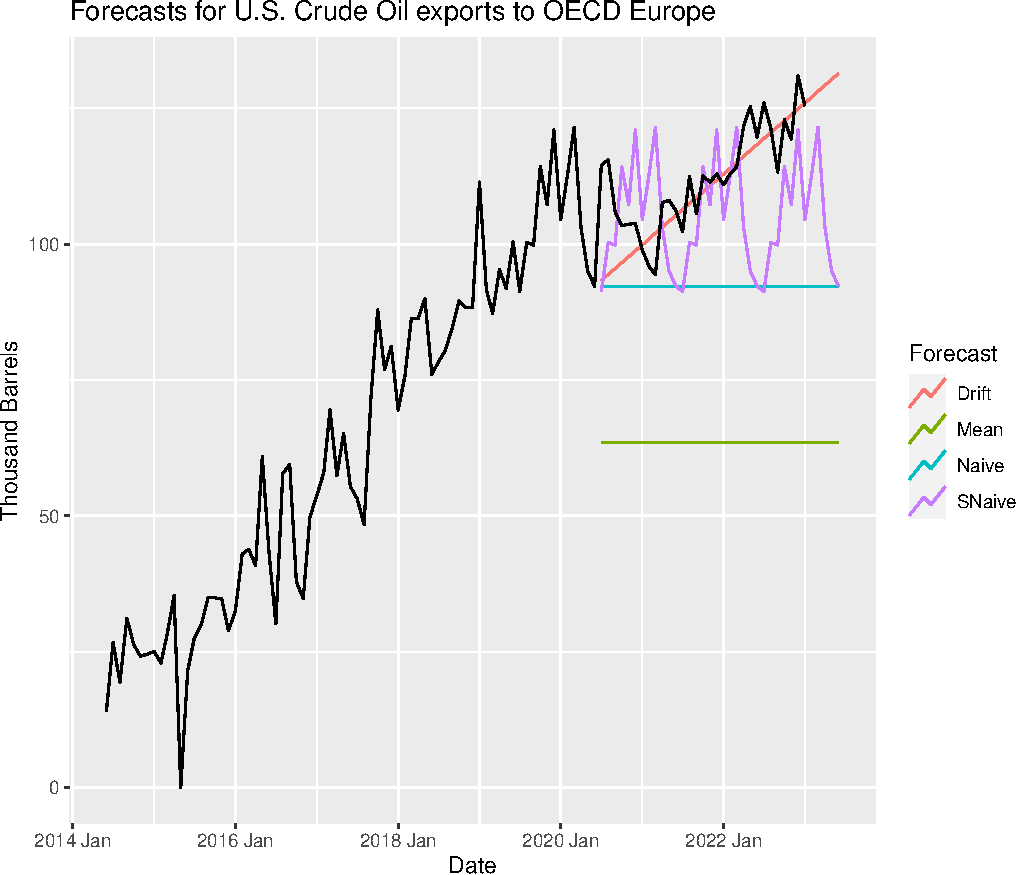
\includegraphics{draft1_files/figure-latex/Forecasting plots-1} \end{center}

\begin{Shaded}
\begin{Highlighting}[]
\NormalTok{nat\_gas\_tr }\OtherTok{\textless{}{-}}\NormalTok{ nat\_gas\_bx }\SpecialCharTok{\%\textgreater{}\%} 
  \FunctionTok{filter}\NormalTok{(Date }\SpecialCharTok{\textless{}=} \FunctionTok{as.Date}\NormalTok{(}\StringTok{"2020{-}06{-}01"}\NormalTok{))}


\NormalTok{nat\_gas\_fit }\OtherTok{\textless{}{-}}\NormalTok{ nat\_gas\_tr }\SpecialCharTok{\%\textgreater{}\%} 
  \FunctionTok{model}\NormalTok{(}
    \AttributeTok{Mean =} \FunctionTok{MEAN}\NormalTok{(Total\_Exports),}
    \AttributeTok{Naive =} \FunctionTok{NAIVE}\NormalTok{(Total\_Exports),}
    \AttributeTok{SNaive =} \FunctionTok{SNAIVE}\NormalTok{(Total\_Exports),}
    \AttributeTok{Drift =} \FunctionTok{RW}\NormalTok{(Total\_Exports }\SpecialCharTok{\textasciitilde{}} \FunctionTok{drift}\NormalTok{())}
\NormalTok{  )}

\NormalTok{nat\_gas\_fc }\OtherTok{\textless{}{-}}\NormalTok{ nat\_gas\_fit }\SpecialCharTok{\%\textgreater{}\%} 
  \FunctionTok{forecast}\NormalTok{(}\AttributeTok{h =} \DecValTok{36}\NormalTok{)}

\NormalTok{nat\_gas\_fc }\SpecialCharTok{\%\textgreater{}\%} 
  \FunctionTok{autoplot}\NormalTok{(}
\NormalTok{    nat\_gas\_bx,}
    \AttributeTok{level =} \ConstantTok{NULL}\NormalTok{) }\SpecialCharTok{+}
  \FunctionTok{labs}\NormalTok{(}
    \AttributeTok{y =} \StringTok{"Amount of natural gas (BOE)"}\NormalTok{,}
    \AttributeTok{title =} \StringTok{"Forecasts for U.S. Natural gas exports to OECD Europe"}\NormalTok{) }\SpecialCharTok{+}
  \FunctionTok{guides}\NormalTok{(}\AttributeTok{colour =} \FunctionTok{guide\_legend}\NormalTok{(}\AttributeTok{title =} \StringTok{"Forecast"}\NormalTok{))}
\end{Highlighting}
\end{Shaded}

\begin{center}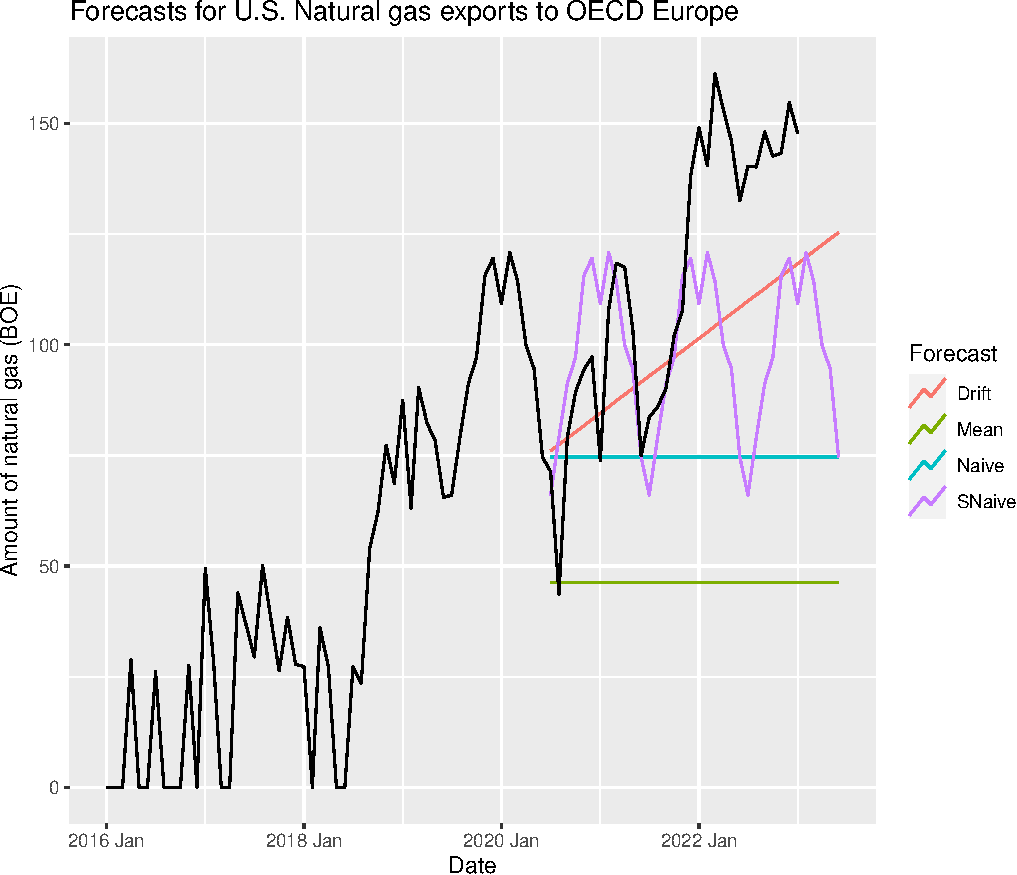
\includegraphics{draft1_files/figure-latex/Forecasting plots-2} \end{center}

Only looking at plots in Figure {[}{]} we can see that our intuition was
right and drift method still seems as most appropriate after conducting
visual inspection. Though, it is important to highlight that if in case
of crude oil exports Drift method was actually quite good at forecasting
export amounts, in the case of natural gas exports Drift method looked
as best of all but still quite far away from actual data. The important
takeaway at this point is the fact that the average growth rate
calculated from historical data was strongly effected by dropped exports
during the COVID pandemic.

After inspecting data visually we will conduct cross validation to see
if our initial predictions that Drift method is most appropriate to
forecast both time series was right.

\begin{Shaded}
\begin{Highlighting}[]
\CommentTok{\#Traditional accuracy}


\NormalTok{accuracy1 }\OtherTok{\textless{}{-}} \FunctionTok{accuracy}\NormalTok{(crude\_oil\_fit) }\SpecialCharTok{\%\textgreater{}\%} 
  \FunctionTok{arrange}\NormalTok{(.model) }\SpecialCharTok{\%\textgreater{}\%} 
  \FunctionTok{select}\NormalTok{(.model, .type, RMSE, MAE, MAPE, MASE, RMSSE)}

\NormalTok{accuracy1}
\end{Highlighting}
\end{Shaded}

\begin{verbatim}
## # A tibble: 4 x 7
##   .model .type     RMSE   MAE  MAPE  MASE RMSSE
##   <chr>  <chr>    <dbl> <dbl> <dbl> <dbl> <dbl>
## 1 Drift  Training  11.3  8.63 Inf   0.509 0.538
## 2 Mean   Training  30.9 27.4  Inf   1.62  1.47 
## 3 Naive  Training  11.4  8.68 Inf   0.512 0.540
## 4 SNaive Training  21.0 17.0   24.7 1     1
\end{verbatim}

\begin{Shaded}
\begin{Highlighting}[]
\NormalTok{accuracy2 }\OtherTok{\textless{}{-}} \FunctionTok{accuracy}\NormalTok{(nat\_gas\_fit) }\SpecialCharTok{\%\textgreater{}\%} 
  \FunctionTok{arrange}\NormalTok{(.model) }\SpecialCharTok{\%\textgreater{}\%} 
  \FunctionTok{select}\NormalTok{(.model, .type, RMSE, MAE, MAPE, MASE, RMSSE)}

\NormalTok{accuracy2}
\end{Highlighting}
\end{Shaded}

\begin{verbatim}
## # A tibble: 4 x 7
##   .model .type     RMSE   MAE  MAPE  MASE RMSSE
##   <chr>  <chr>    <dbl> <dbl> <dbl> <dbl> <dbl>
## 1 Drift  Training  19.3  15.4   Inf 0.439 0.489
## 2 Mean   Training  38.3  33.3   Inf 0.946 0.972
## 3 Naive  Training  19.3  15.1   Inf 0.430 0.490
## 4 SNaive Training  39.4  35.2   Inf 1     1
\end{verbatim}

\begin{Shaded}
\begin{Highlighting}[]
\CommentTok{\#Time series cross validation}

\NormalTok{crude\_oil\_tr2 }\OtherTok{\textless{}{-}}\NormalTok{ crude\_oil\_bx }\SpecialCharTok{\%\textgreater{}\%}
\FunctionTok{stretch\_tsibble}\NormalTok{(}\AttributeTok{.init =} \DecValTok{3}\NormalTok{, }\AttributeTok{.step =} \DecValTok{1}\NormalTok{) }\SpecialCharTok{\%\textgreater{}\%}
\FunctionTok{relocate}\NormalTok{(Date,Total\_Exports, .id)}

\NormalTok{crude\_oil\_tr2 }\SpecialCharTok{\%\textgreater{}\%}
\FunctionTok{model}\NormalTok{(}\AttributeTok{Drift =} \FunctionTok{RW}\NormalTok{(Total\_Exports }\SpecialCharTok{\textasciitilde{}} \FunctionTok{drift}\NormalTok{())) }\SpecialCharTok{\%\textgreater{}\%}
\FunctionTok{forecast}\NormalTok{(}\AttributeTok{h =} \DecValTok{12}\NormalTok{) }\SpecialCharTok{\%\textgreater{}\%}
\FunctionTok{accuracy}\NormalTok{(crude\_oil\_bx)}
\end{Highlighting}
\end{Shaded}

\begin{verbatim}
## # A tibble: 1 x 10
##   .model .type    ME  RMSE   MAE   MPE  MAPE  MASE RMSSE  ACF1
##   <chr>  <chr> <dbl> <dbl> <dbl> <dbl> <dbl> <dbl> <dbl> <dbl>
## 1 Drift  Test  -2.03  14.9  10.9  -Inf   Inf 0.708 0.786 0.716
\end{verbatim}

\begin{Shaded}
\begin{Highlighting}[]
\NormalTok{crude\_oil\_bx }\SpecialCharTok{|\textgreater{}}
  \FunctionTok{model}\NormalTok{(}\FunctionTok{RW}\NormalTok{(Total\_Exports }\SpecialCharTok{\textasciitilde{}} \FunctionTok{drift}\NormalTok{())) }\SpecialCharTok{|\textgreater{}}
  \FunctionTok{accuracy}\NormalTok{()}
\end{Highlighting}
\end{Shaded}

\begin{verbatim}
## # A tibble: 1 x 10
##   .model              .type        ME  RMSE   MAE   MPE  MAPE  MASE RMSSE   ACF1
##   <chr>               <chr>     <dbl> <dbl> <dbl> <dbl> <dbl> <dbl> <dbl>  <dbl>
## 1 RW(Total_Exports ~~ Trai~ -3.97e-15  10.2  7.65  -Inf   Inf 0.496 0.539 -0.319
\end{verbatim}

\hypertarget{residual-diagnostics}{%
\paragraph{4.3. Residual diagnostics}\label{residual-diagnostics}}

First we inspect residuals of drift and naive methods for crude oil
exports.Both, according to previous analysis were most accurate.

\begin{Shaded}
\begin{Highlighting}[]
\CommentTok{\#Inspecting residuals crude oil}

\NormalTok{drift\_crude\_oil }\OtherTok{\textless{}{-}}\NormalTok{ crude\_oil\_tr }\SpecialCharTok{\%\textgreater{}\%} 
  \FunctionTok{model}\NormalTok{(}\FunctionTok{RW}\NormalTok{(Total\_Exports }\SpecialCharTok{\textasciitilde{}} \FunctionTok{drift}\NormalTok{()))}

\NormalTok{naive\_crude\_oil }\OtherTok{\textless{}{-}}\NormalTok{ crude\_oil\_tr }\SpecialCharTok{\%\textgreater{}\%} 
  \FunctionTok{model}\NormalTok{(}\FunctionTok{NAIVE}\NormalTok{(Total\_Exports))}

\FunctionTok{gg\_tsresiduals}\NormalTok{(drift\_crude\_oil)}
\end{Highlighting}
\end{Shaded}

\begin{center}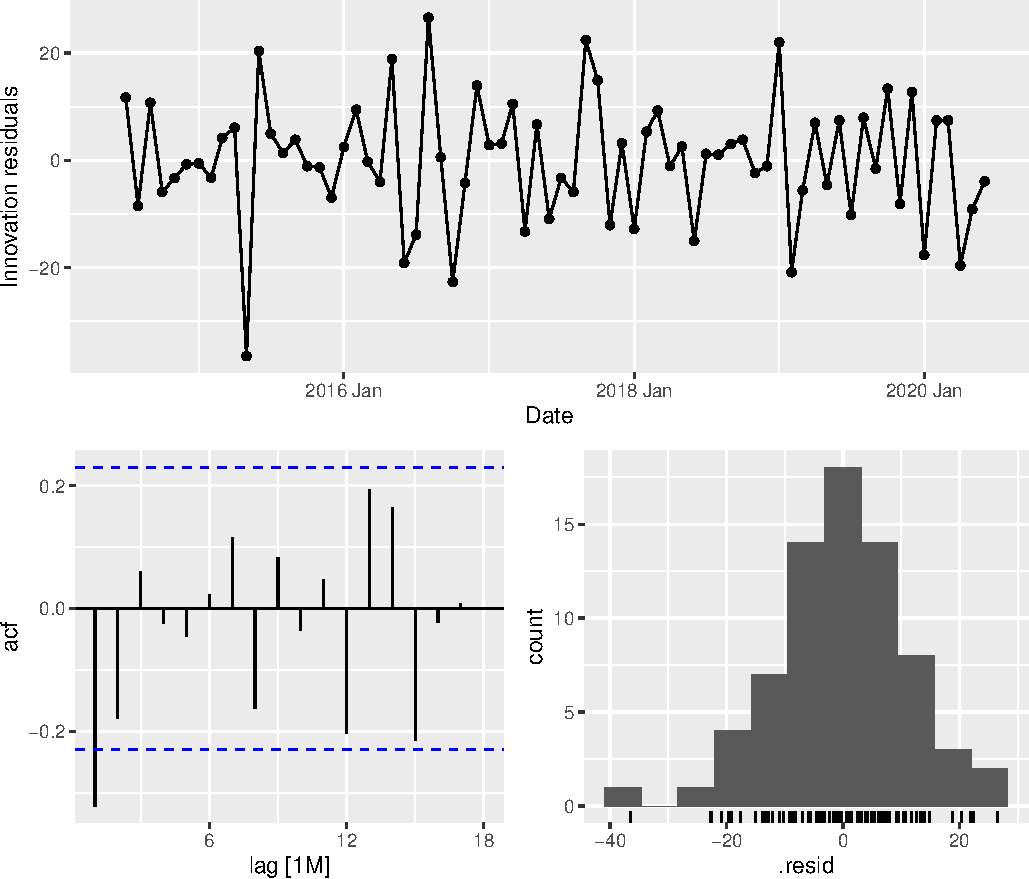
\includegraphics{draft1_files/figure-latex/Residual diagnostics (crude oil)-1} \end{center}

\begin{Shaded}
\begin{Highlighting}[]
\FunctionTok{gg\_tsresiduals}\NormalTok{(naive\_crude\_oil)}
\end{Highlighting}
\end{Shaded}

\begin{center}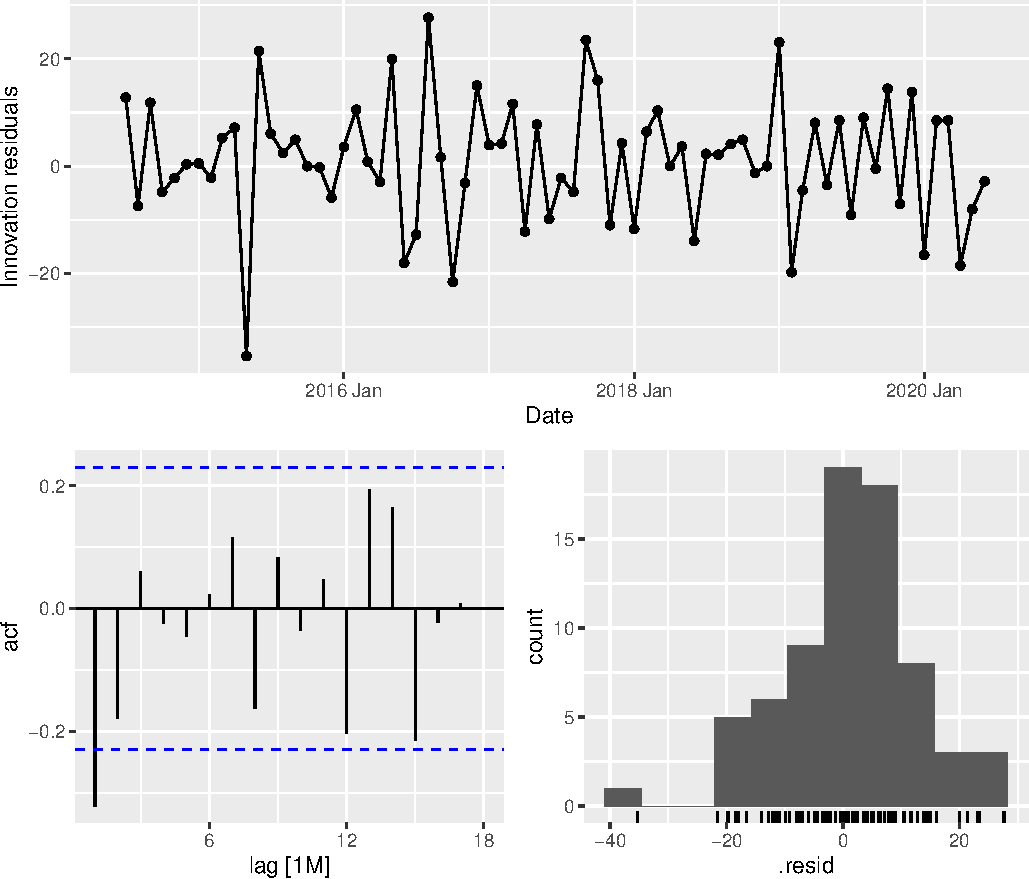
\includegraphics{draft1_files/figure-latex/Residual diagnostics (crude oil)-2} \end{center}

The graphs demonstrate that the naive and drift forecasting methods
providecrude oil export predictions that seem to capture all the
relevant information available. The residuals, or the differences
between the predicted values and actual values, have a mean close to
zero and do not show any significant correlation, as evidenced by the
lack of discernible patterns in the residual series. The time plot of
the residuals indicates that their variance remains relatively constant
across the historical data, except for one outlier at the beginning of
the time series (which corresponds to the zeros observed during that
time period). This constant residual variance is further supported by
the histogram of the residuals.

We conduct the same analysis with drift and naive methods on natural gas
exports.

\begin{Shaded}
\begin{Highlighting}[]
\CommentTok{\#Inspecting residuals nat gas}

\NormalTok{drift\_nat\_gas }\OtherTok{\textless{}{-}}\NormalTok{ nat\_gas\_bx }\SpecialCharTok{\%\textgreater{}\%} 
  \FunctionTok{model}\NormalTok{(}\FunctionTok{RW}\NormalTok{(Total\_Exports }\SpecialCharTok{\textasciitilde{}} \FunctionTok{drift}\NormalTok{()))}

\NormalTok{naive\_nat\_gas }\OtherTok{\textless{}{-}}\NormalTok{ nat\_gas\_bx }\SpecialCharTok{\%\textgreater{}\%} 
  \FunctionTok{model}\NormalTok{(}\FunctionTok{NAIVE}\NormalTok{(Total\_Exports))}

\FunctionTok{gg\_tsresiduals}\NormalTok{(drift\_nat\_gas)}
\end{Highlighting}
\end{Shaded}

\begin{center}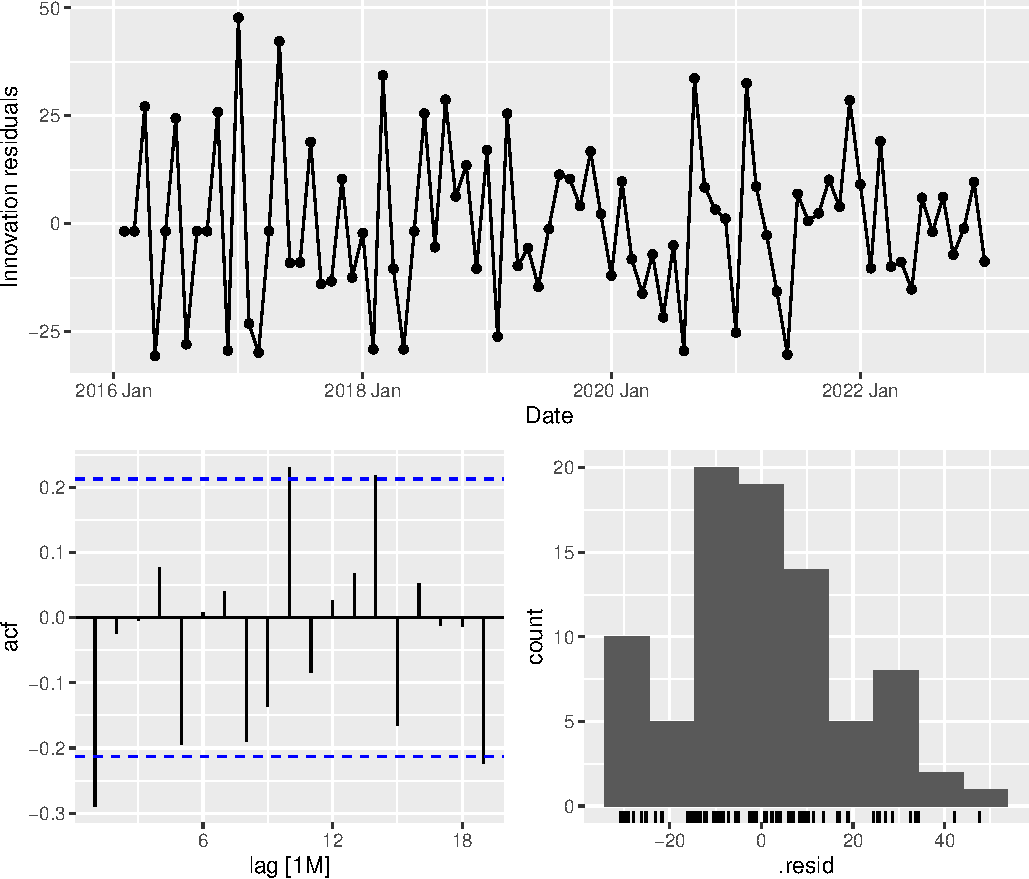
\includegraphics{draft1_files/figure-latex/Residual diagnostics (nat gas)-1} \end{center}

\begin{Shaded}
\begin{Highlighting}[]
\FunctionTok{gg\_tsresiduals}\NormalTok{(naive\_nat\_gas)}
\end{Highlighting}
\end{Shaded}

\begin{center}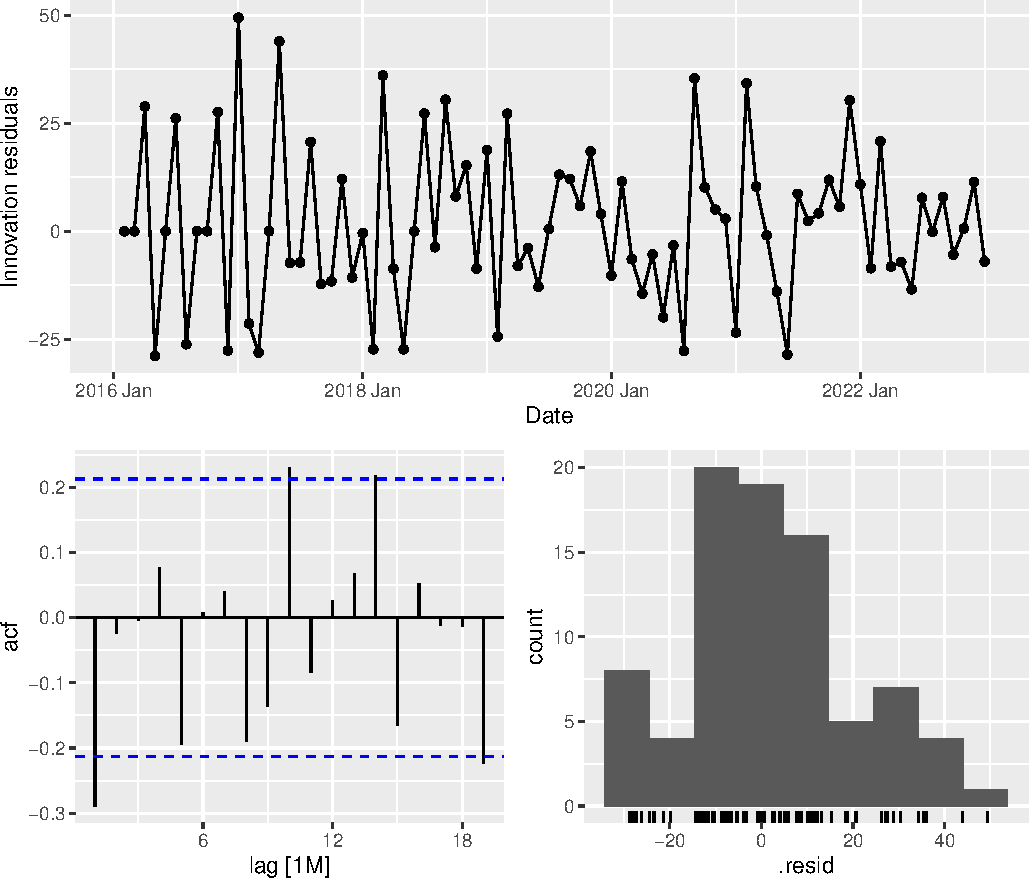
\includegraphics{draft1_files/figure-latex/Residual diagnostics (nat gas)-2} \end{center}

Looking at the graphs we see that in cases of both methods the residuals
seem to stay close to zero therefore implying that there is no
correlation between the residuals and thus suggesting that the models
are accurate in the predictions of the data.

\hypertarget{exponential-smoothing}{%
\subsection{5. Exponential smoothing}\label{exponential-smoothing}}

Yet to be started

\hypertarget{arima}{%
\subsection{6. ARIMA}\label{arima}}

Yet to be started

\hypertarget{other-forecasting-methods}{%
\subsection{7. Other forecasting
methods}\label{other-forecasting-methods}}

Yet to be started

\end{document}
